% ============================================================
% BÁO CÁO BÀI TẬP LỚN ET3161 — Phân tích và Thiết kế Hệ thống Phần mềm
% Hệ thống hỗ trợ Quy trình Quản lý Trang thiết bị QT.QLD.09.01
% Biên dịch: xelatex main.tex (chạy 2 lần để cập nhật mục lục)
% ============================================================
\documentclass[12pt, a4paper]{report}

\usepackage[margin=2.5cm, top=2.8cm, bottom=2.8cm]{geometry}
\usepackage{fontspec}
\usepackage{setspace}
\usepackage{graphicx}
\usepackage{booktabs}
\usepackage{amssymb}
\usepackage{longtable}
\usepackage{array}
\usepackage{xcolor}
\usepackage{enumitem}
\usepackage{fancyhdr}
\usepackage{titlesec}
\usepackage{caption}
\usepackage[hidelinks, unicode]{hyperref}

% ---- Font hỗ trợ tiếng Việt (có sẵn trên Windows) ----
\setmainfont{Times New Roman}
\setsansfont{Arial}

\onehalfspacing
\setlist{nosep, leftmargin=2em}

% ---- Tiêu đề chương/section ----
\titleformat{\chapter}[display]
  {\normalfont\Large\bfseries\centering}{Chương \thechapter}{6pt}{\Large}
\titlespacing*{\chapter}{0pt}{-10pt}{16pt}

% ---- Header/footer ----
\pagestyle{fancy}
\fancyhf{}
\fancyhead[L]{\small\leftmark}
\fancyhead[R]{\small Bài tập lớn ET3161}
\fancyfoot[C]{\thepage}
\renewcommand{\headrulewidth}{0.3pt}

% ---- Bảng ----
\renewcommand{\arraystretch}{1.25}
\captionsetup{font=small, labelfont=bf}

\newcolumntype{P}[1]{>{\raggedright\arraybackslash}p{#1}}

% ---- Tiếng Việt hóa các nhãn mặc định ----
\renewcommand{\contentsname}{Mục lục}
\renewcommand{\listfigurename}{Danh mục hình}
\renewcommand{\listtablename}{Danh mục bảng}
\renewcommand{\chaptermark}[1]{\markboth{Chương \thechapter.\ #1}{}}

\begin{document}

% ================= TRANG BÌA =================
\begin{titlepage}
\centering
{\Large \textbf{TRƯỜNG ĐẠI HỌC BÁCH KHOA HÀ NỘI}}\\[2pt]
{\large Viện Công nghệ Thông tin và Truyền thông}\\[40pt]
{\Huge\bfseries BÁO CÁO BÀI TẬP LỚN}\\[10pt]
{\Large Môn: Phân tích và Thiết kế Hệ thống Phần mềm (ET3161)}\\[36pt]
\begin{minipage}{0.86\textwidth}
\centering
{\Large\bfseries HỆ THỐNG HỖ TRỢ QUY TRÌNH\\ QUẢN LÝ TRANG THIẾT BỊ (QT.QLD.09.01)\\[6pt]
CỤC QUẢN LÝ DƯỢC — BỘ Y TẾ}\\[14pt]
{\large Số hóa biểu mẫu BM.QLD.09.01/01 $\rightarrow$ /04\\ theo chuẩn UML và cài đặt thử nghiệm}
\end{minipage}\\[60pt]
\begin{flushright}
\begin{tabular}{ll}
\textbf{Sinh viên thực hiện:} & \\[4pt]
Họ và tên: & \underline{\hspace{6cm}} \\[8pt]
MSSV: & \underline{\hspace{6cm}} \\[8pt]
Lớp: & \underline{\hspace{6cm}} \\[8pt]
Giảng viên hướng dẫn: & \underline{\hspace{6cm}} \\
\end{tabular}
\end{flushright}
\vfill
{\large Hà Nội --- 2026}
\end{titlepage}

% ================= MỤC LỤC =================
\tableofcontents
\listoffigures
\listoftables

% ================= CÁC CHƯƠNG =================
\chapter{Giới thiệu đề tài}

\section{Bối cảnh}

Cục Quản lý Dược (Bộ Y tế) vận hành Hệ thống quản lý chất lượng (HT QLCL) theo TCVN ISO 9001:2015. Trong khuôn khổ đó, quy trình \textbf{QT.QLD.09.01 --- Quản lý trang thiết bị} (ban hành 07/8/2018, lần ban hành 01, biên soạn bởi Thư ký QMS, kiểm tra bởi Lãnh đạo chất lượng, phê duyệt bởi Cục trưởng) quy định cách thức thống nhất trong việc quản lý trang thiết bị của Cục nhằm:
\begin{itemize}
  \item duy trì sự hoạt động ổn định, liên tục của các trang thiết bị;
  \item đảm bảo độ tin cậy của các thiết bị;
  \item phòng ngừa, ngăn chặn sự cố;
  \item hạn chế thiệt hại đến mức thấp nhất nếu sự cố xảy ra.
\end{itemize}

Quy trình hiện đang vận hành thủ công qua bốn biểu mẫu giấy/Excel:
\begin{itemize}
  \item \textbf{BM.QLD.09.01/01} --- Danh mục trang thiết bị;
  \item \textbf{BM.QLD.09.01/02} --- Hồ sơ trang thiết bị (lịch sử bảo trì, sửa chữa);
  \item \textbf{BM.QLD.09.01/03} --- Kế hoạch bảo dưỡng, thay thế hàng năm;
  \item \textbf{BM.QLD.09.01/04} --- Biên bản nghiệm thu.
\end{itemize}

\section{Vấn đề của quy trình thủ công}

Qua khảo sát tài liệu quy trình và đối chiếu thực tiận vận hành, nhóm xác định các hạn chế chính của quy trình giấy (chi tiết tại mục 2.5):
\begin{enumerate}
  \item Hồ sơ thiết bị phân tán tại từng đơn vị sử dụng, khó tổng hợp và dễ thất lạc.
  \item Việc cập nhật hồ sơ (BM/02) phụ thuộc kỷ luật nhập liệu thủ công, thiếu cơ chế ép buộc, dẫn đến thiếu vết truy vết khi cần kiểm tra của Ban QMS.
  \item Kế hoạch bảo dưỡng hàng năm (BM/03) lưu tại Văn phòng Cục với thời hạn 1 năm; không có cơ chế nhắc lịch, dễ bỏ sót hạng mục đến hạn.
  \item Luồng phê duyệt bằng văn bản giấy (đơn vị $\rightarrow$ Văn phòng Cục $\rightarrow$ Lãnh đạo Cục) kéo dài thời gian, không theo dõi được trạng thái xử lý.
  \item Biên bản nghiệm thu (BM/04) lưu 1 năm tại đơn vị sử dụng, khó tra cứu khi phát sinh tranh chấp với nhà thầu.
\end{enumerate}

\section{Mục tiêu của hệ thống}

Hệ thống phần mềm được phân tích và thiết kế trong báo cáo này nhằm:
\begin{enumerate}
  \item \textbf{Số hóa} toàn bộ bốn biểu mẫu thành dữ liệu có cấu trúc, tránh thất lạc, trùng lặp.
  \item \textbf{Tự động hóa luồng phê duyệt} (đơn vị $\rightarrow$ Văn phòng Cục $\rightarrow$ Lãnh đạo Cục) với trạng thái theo dõi thời gian thực.
  \item \textbf{Cảnh báo, nhắc lịch} bảo dưỡng định kỳ, tránh bỏ sót.
  \item \textbf{Truy vết đầy đủ} lịch sử sự cố --- sửa chữa --- nghiệm thu của từng thiết bị; dữ liệu lịch sử chỉ thêm, không sửa/xóa (audit trail).
  \item \textbf{Báo cáo, thống kê} cho Ban QMS và Lãnh đạo Cục.
\end{enumerate}

\section{Phạm vi}

\textbf{Trong phạm vi:} quản lý danh mục trang thiết bị; hồ sơ thiết bị; báo và xử lý sự cố (nhỏ — tự khắc phục, lớn — thuê ngoài có phê duyệt); kế hoạch bảo dưỡng hàng năm và nhắc lịch; biên bản nghiệm thu; quản lý nhà thầu; phân quyền theo vai trò; báo cáo thống kê; nhật ký thao tác.

\textbf{Ngoài phạm vi:} quản lý tài sản hữu hình ngoài trang thiết bị (mô hình kế toán); thanh toán hợp đồng với nhà thầu; quản lý cơ sở hạ tầng (bản quy trình được đính kèm với tên file có ``và CSHT'' nhưng nội dung lần ban hành 01 chỉ đề cập trang thiết bị); tích hợp chữ ký số thực (hệ thống mô phỏng ký điện tử); SSO/Active Directory (kế hoạch mở rộng).

\section{Phương pháp phân tích và thiết kế}

Nhóm áp dụng quy trình phân tích thiết kế hướng đối tượng theo tài liệu [3], [4]:
\begin{itemize}
  \item \textbf{Xác định yêu cầu:} khảo sát quy trình gốc, phỏng vấn ảo theo vai trò, trích xuất trường dữ liệu từ bốn biểu mẫu.
  \item \textbf{Mô hình hóa chức năng (Chương 3):} sơ đồ use case, đặc tả use case, sơ đồ hoạt động có phân làn.
  \item \textbf{Mô hình hóa cấu trúc (Chương 4):} phân tích danh từ — động từ để xác định lớp, sơ đồ lớp, thẻ CRC.
  \item \textbf{Mô hình hóa hành vi (Chương 5):} sơ đồ trình tự, sơ đồ trạng thái.
  \item \textbf{Thiết kế (Chương 6):} kiến trúc ba lớp, thiết kế cơ sở dữ liệu quan hệ, thiết kế giao diện, thiết kế bảo mật.
  \item \textbf{Cài đặt thử nghiệm (Chương 7):} nguyên mẫu chạy được, triển khai Docker Compose.
\end{itemize}

Một nguyên tắc xuyên suốt của nhóm: \emph{giữ đúng ngữ nghĩa nghiệp vụ của quy trình gốc} — đặc biệt là nhánh ``sự cố nhỏ đơn vị tự khắc phục'' không bắt buộc qua phê duyệt đầy đủ — đồng thời tách bạch rõ các tính năng mở rộng (chi phí, mức độ ưu tiên, nhà thầu, SLA) so với nội dung nguyên bản.

\chapter{Khảo sát và phân tích yêu cầu}

\section{Mô tả quy trình hiện tại (As-is)}

\subsection{Vai trò và trách nhiệm}

Theo mục 4 và mục 6.2 của quy trình QT.QLD.09.01, các vai trò tham gia được tổng hợp trong Bảng~\ref{tab:vaitro}.

\begin{table}[h]
\centering
\caption{Vai trò và trách nhiệm theo quy trình gốc}
\label{tab:vaitro}
\begin{tabular}{P{3.4cm}P{11.6cm}}
\toprule
\textbf{Vai trò} & \textbf{Trách nhiệm chính} \\
\midrule
Đơn vị sử dụng & Xây dựng, cập nhật danh mục và hồ sơ trang thiết bị của đơn vị; thông báo sự cố/nguy cơ sự cố cho Văn phòng Cục; tự khắc phục sự cố nhỏ và cập nhật hồ sơ; phối hợp thực hiện, theo dõi giám sát, nghiệm thu; lưu biên bản nghiệm thu \\
Văn phòng Cục & Lập danh mục tổng toàn Cục (BM/01); cập nhật danh mục và hồ sơ sau sự cố/sửa chữa; lập kế hoạch bảo dưỡng hàng năm (BM/03) hoặc tiếp nhận văn bản đề nghị; trình Lãnh đạo Cục phê duyệt; kiểm tra nguyên nhân sự cố; liên hệ đơn vị ngoài; theo dõi giám sát; lập biên bản nghiệm thu (BM/04); lưu hồ sơ \\
Lãnh đạo Cục & Phê duyệt kế hoạch bảo dưỡng/thay thế, phương án bổ sung/nâng cấp, phương án sửa chữa thuê ngoài \\
Lãnh đạo chất lượng, Ban QMS & Kiểm tra, bảo đảm quy trình được thực hiện và tuân thủ \\
Bên ngoài (Công ty) & Thực hiện bảo dưỡng/sửa chữa/thay thế khi được thuê; tham gia ký biên bản nghiệm thu (Bên B) \\
\bottomrule
\end{tabular}
\end{table}

\subsection{Luồng nghiệp vụ chính}

Quy trình gồm năm nhóm bước (mục 6.2 của quy trình):

\begin{enumerate}
  \item \textbf{6.2.1 Lập danh mục trang thiết bị:} Văn phòng Cục xây dựng danh mục toàn Cục; bổ sung thiết bị mới, cập nhật tình trạng sau sự cố/sửa chữa; các đơn vị xây dựng và cập nhật danh mục của đơn vị. Sử dụng BM/01.
  \item \textbf{6.2.2 Xây dựng hồ sơ trang thiết bị:} đơn vị sử dụng xây dựng hồ sơ, cập nhật khi có sự cố, sửa chữa, thay thế, bảo dưỡng. Sử dụng BM/02.
  \item \textbf{6.2.3 Bảo dưỡng, sửa chữa:} hai nhánh song song:
  \begin{itemize}
    \item (a) \emph{Hàng năm}, Văn phòng Cục lập kế hoạch bảo dưỡng định kỳ hoặc đề xuất bổ sung, nâng cấp $\rightarrow$ trình Lãnh đạo Cục phê duyệt (BM/03). Thiết bị cần bảo dưỡng ngoài kế hoạch hoặc đơn vị cần bổ sung/nâng cấp: gửi văn bản cho Văn phòng Cục trình duyệt.
    \item (b) \emph{Sửa chữa khi có sự cố:} đơn vị thông báo cho Văn phòng Cục xem xét. \textbf{Sự cố nhỏ khắc phục ngay được: đơn vị tự khắc phục và cập nhật hồ sơ (không cần phê duyệt).} Không tự khắc phục được, cần thuê ngoài: lập văn bản đề nghị $\rightarrow$ Văn phòng Cục trình Lãnh đạo Cục phê duyệt.
  \end{itemize}
  \item \textbf{6.2.4 Thực hiện:} theo kế hoạch hoặc phương án đã duyệt; Văn phòng Cục phối hợp đơn vị sử dụng tiến hành và cập nhật danh sách, hồ sơ thiết bị. Trong bảo dưỡng nếu phát hiện nguyên nhân tiềm tàng gây sự cố thì báo lại để đề xuất phương án sửa chữa, thay thế.
  \item \textbf{6.2.5 Kiểm tra, nghiệm thu:} khi thuê ngoài — theo dõi, giám sát; kiểm tra, chạy thử sau khi kết thúc; lập biên bản nghiệm thu (BM/04); cập nhật hồ sơ thiết bị.
\end{enumerate}

\subsection{Điểm quyết định then chốt}

Điểm rẽ nhánh quan trọng nhất của lưu đồ nằm sau bước ``Kiểm tra, xem xét nguyên nhân'':
\begin{itemize}
  \item \textbf{[Sự cố nhỏ]} $\rightarrow$ Tự khắc phục $\rightarrow$ cập nhật hồ sơ $\rightarrow$ kết thúc. \emph{Không} đi qua phê duyệt.
  \item \textbf{[Lớn / cần thuê ngoài]} $\rightarrow$ Lập phương án sửa chữa (hoặc kế hoạch thay thế, bảo dưỡng) $\rightarrow$ \textbf{Phê duyệt (Lãnh đạo Cục)} $\rightarrow$ Thực hiện $\rightarrow$ Kiểm tra, nghiệm thu $\rightarrow$ Lưu hồ sơ.
\end{itemize}
Thiết kế hệ thống ở Chương 6 tái hiện đúng cấu trúc này: nhánh nhỏ chỉ cập nhật hồ sơ, nhánh lớn bắt buộc qua state machine phê duyệt.

\section{Trường dữ liệu của bốn biểu mẫu}

Nhóm trích xuất toàn văn quy trình gốc và xác minh nguyên văn các trường dữ liệu (đây là nguồn dữ liệu để thiết kế CSDL ở Chương 6).

\begin{table}[h]
\centering
\caption{Trường dữ liệu của các biểu mẫu BM.QLD.09.01/01--/04}
\label{tab:bieumau}
\begin{tabular}{P{3.1cm}P{11.9cm}}
\toprule
\textbf{Biểu mẫu} & \textbf{Trường dữ liệu (nguyên văn)} \\
\midrule
BM/01 --- Danh mục trang thiết bị & STT; Tên trang thiết bị; Mã số; Nước sản xuất; Ngày nhận; Đơn vị sử dụng \\
\addlinespace
BM/02 --- Hồ sơ trang thiết bị & Thông tin đầu: Tên trang thiết bị; Ngày nhận; Mã số; Đơn vị sử dụng. Bảng lịch sử: STT; Ngày thực hiện; Nội dung bảo trì, sửa chữa; Người thực hiện \\
\addlinespace
BM/03 --- Kế hoạch bảo dưỡng, thay thế & Năm; STT; Tên trang thiết bị; Mã số; Đơn vị sử dụng; Nội dung; Đơn vị thực hiện (nội bộ/bên ngoài); Thời gian dự kiến (tháng); Ghi chú. Chữ ký: Văn phòng Cục và Lãnh đạo Cục \\
\addlinespace
BM/04 --- Biên bản nghiệm thu & Quốc hiệu, tiêu ngữ; Hà Nội, ngày... tháng... năm...; Đại diện Cục Quản lý Dược (Bên A): 2 người (Họ tên, Đơn vị); Đại diện Công ty (Bên B): 2 người (Họ tên, Đơn vị); ``Bên B đã thực hiện... các nội dung công việc sau''; ``Tình trạng hoạt động của trang thiết bị sau khi Bên B thực hiện''; ``Lập thành 02 bản, mỗi bên giữ 01 bản''. Chữ ký hai bên \\
\bottomrule
\end{tabular}
\end{table}

\textbf{Nhận xét khảo sát:} (i) nguyên bản \emph{không có} trường chi phí, mức độ ưu tiên hay danh mục mã hóa tình trạng — hệ thống bổ sung các trường này như ``mở rộng đề xuất'' (đánh dấu rõ ở Chương 6); (ii) biên bản BM/04 của nguyên bản có lỗi đánh máy ở phần chữ ký (cả hai bên đều ghi ``BÊN B'') — hệ thống chuẩn hóa thành ``BÊN A'' (Cục Quản lý Dược) và ``BÊN B'' (Công ty); (iii) tên file tài liệu đính kèm có ``và CSHT'' nhưng nội dung lần ban hành 01 không đề cập cơ sở hạ tầng.

\section{Quy định lưu trữ hồ sơ (mục 7)}

\begin{table}[h]
\centering
\caption{Hồ sơ, nơi lưu và thời hạn lưu trữ theo mục 7 của quy trình}
\label{tab:luutru}
\begin{tabular}{P{6.2cm}P{2.8cm}P{2.4cm}P{3.4cm}}
\toprule
\textbf{Tên hồ sơ} & \textbf{Ký hiệu} & \textbf{Nơi lưu} & \textbf{Thời gian lưu} \\
\midrule
Danh mục trang thiết bị & BM.QLD.09.01/01 & Văn phòng Cục, Đơn vị sử dụng & Đến lần cập nhật tiếp theo \\
Hồ sơ trang thiết bị & BM.QLD.09.01/02 & Đơn vị sử dụng & Đến khi máy không sử dụng \\
Kế hoạch bảo dưỡng, thay thế & BM.QLD.09.01/03 & Văn phòng Cục & 1 năm \\
Biên bản nghiệm thu & BM.QLD.09.01/04 & Đơn vị sử dụng & 1 năm \\
\bottomrule
\end{tabular}
\end{table}

Hệ thống điện tử áp dụng các thời hạn này ở tầng ứng dụng (cảnh báo hết hạn lưu trữ) và tách bạch với nguyên tắc truy vết của ISO 9001: dữ liệu nghiệp vụ được giữ vết qua nhật ký (audit trail) append-only; thời hạn lưu trữ quy định việc lưu hồ sơ biểu mẫu tương ứng.

\section{Phân tích vấn đề và yêu cầu}

\subsection{Vấn đề (Problems)}

\begin{table}[h]
\centering
\caption{Vấn đề của quy trình giấy và hệ quả}
\label{tab:vande}
\begin{tabular}{P{0.8cm}P{6.2cm}P{8cm}}
\toprule
\textbf{STT} & \textbf{Vấn đề} & \textbf{Hệ quả} \\
\midrule
P1 & Hồ sơ phân tán tại đơn vị, quản lý bằng giấy/Excel & Khó tổng hợp, mất đồng bộ giữa danh mục đơn vị và danh mục Văn phòng Cục \\
P2 & Cập nhật hồ sơ BM/02 thủ công, không bắt buộc & Thiếu vết truy vết, Ban QMS khó kiểm tra tuân thủ \\
P3 & Không có nhắc lịch bảo dưỡng & Bỏ sót hạng mục đến hạn, thiết bị hỏng ngoài dự kiến \\
P4 & Phê duyệt bằng văn bản giấy & Chậm, không thấy trạng thái, khó đôn đốc \\
P5 & Nghiệm thu lưu 1 năm tại đơn vị & Khó tra cứu khi tranh chấp nhà thầu, không thống kê được chi phí \\
\bottomrule
\end{tabular}
\end{table}

\subsection{Yêu cầu chức năng}

\begin{longtable}{P{1.6cm}P{8.6cm}P{2cm}P{2.6cm}}
\caption{Danh mục yêu cầu chức năng}\label{tab:fr}\\
\toprule
\textbf{Mã} & \textbf{Yêu cầu} & \textbf{Vấn đề giải quyết} & \textbf{Quy trình gốc} \\
\midrule
\endfirsthead
\toprule
\textbf{Mã} & \textbf{Yêu cầu} & \textbf{Vấn đề} & \textbf{6.2.x} \\
\midrule
\endhead
FR-01 & Quản lý danh mục thiết bị: thêm, sửa, lọc theo tình trạng/đơn vị, tìm kiếm, xuất Excel theo đúng cột BM/01 & P1 & 6.2.1 \\
FR-02 & Hồ sơ thiết bị điện tử: timeline lịch sử bảo trì/sửa chữa theo BM/02, tự ghi bản ghi khi hoàn thành khắc phục/bảo dưỡng/nghiệm thu & P2 & 6.2.2 \\
FR-03 & Báo sự cố trực tuyến (kể cả thiết bị di động), kèm mức độ ước lượng của đơn vị & P3 & 6.2.3b \\
FR-04 & Xem xét nguyên nhân và phân loại xử lý: tự khắc phục / nội bộ / thuê ngoài & P4 & 6.2.3b \\
FR-05 & Luồng tự khắc phục: đơn vị ghi nội dung khắc phục $\rightarrow$ hệ thống tự cập nhật hồ sơ và đóng sự cố, \textbf{không qua phê duyệt} & P4 & 6.2.3b \\
FR-06 & Lập phương án sửa chữa khi thuê ngoài, trình Lãnh đạo Cục phê duyệt/từ chối (kèm lý do) & P4 & 6.2.3b \\
FR-07 & Lập kế hoạch bảo dưỡng hàng năm (nhiều hạng mục), trình duyệt, phê duyệt/từ chối, theo dõi tiến độ từng hạng mục & P3, P4 & 6.2.3a \\
FR-08 & Nhắc lịch tự động: hạng mục dự kiến trong tháng chưa hoàn thành $\rightarrow$ thông báo Văn phòng Cục và đơn vị & P3 & 6.2.3a \\
FR-09 & Nghiệm thu điện tử theo BM/04: lập biên bản, quản lý đại diện hai bên, ký điện tử, đủ chữ ký $\rightarrow$ đóng sự cố + cập nhật hồ sơ + thiết bị về hoạt động & P5 & 6.2.5 \\
FR-10 & Quản lý nhà thầu ngoài (thêm mới, thông tin liên hệ) & P5 & (mở rộng) \\
FR-11 & Báo cáo thống kê: thiết bị theo đơn vị, tình trạng, tần suất sự cố, tiến độ kế hoạch, chi phí dự kiến & P1--P5 & (mở rộng) \\
FR-12 & Phân quyền theo vai trò; đăng nhập nội bộ & P2 & mục 4 \\
FR-13 & Nhật ký thao tác append-only phục vụ kiểm soát tài liệu ISO 9001 & P2 & (ISO) \\
\bottomrule
\end{longtable}

\subsection{Yêu cầu phi chức năng}

\begin{enumerate}[label=\textbf{NFR-\arabic*.}]
  \item \textbf{Truy vết:} dữ liệu lịch sử (hồ sơ thiết bị, audit log) chỉ thêm, không sửa/xóa.
  \item \textbf{Bảo mật:} mật khẩu băm bcrypt; phiên JWT 8 giờ; phân quyền chặt theo vai trò ở tầng API.
  \item \textbf{Tính khả dụng:} giao diện web responsive, dùng tốt trên điện thoại để báo sự cố tại chỗ.
  \item \textbf{Sao lưu:} dữ liệu nằm trong volume Docker; kịch bản \texttt{pg\_dump} hằng ngày; thời hạn lưu trữ theo Bảng~\ref{tab:luutru}.
  \item \textbf{Khả năng mở rộng:} kiến trúc module + REST API, sẵn sàng tích hợp hệ thống quản lý tài sản hoặc SSO/AD sau này.
  \item \textbf{Hiệu năng:} đáp ứng tra cứu danh mục vài trăm thiết bị toàn Cục trong thời gian ngắn hơn 1 giây (mức lý thuyết, chưa đo lường chính thức).
\end{enumerate}

\section{Phân tích độ khả thi}

\begin{itemize}
  \item \textbf{Kỹ thuật:} quy mô nhỏ (vài trăm thiết bị, vài chục người dùng nội bộ), dữ liệu có cấu trúc bảng biểu rõ ràng $\rightarrow$ kiến trúc web ba lớp với CSDL quan hệ (PostgreSQL) là phù hợp; không cần workflow engine nặng, dùng state machine đơn giản trong mã nguồn.
  \item \textbf{Kinh tế:} chi phí hạ tầng thấp (1 máy chủ nội bộ hoặc VPS, Docker); chi phí phát triển thuộc phạm vi bài tập lớn; lợi ích giảm mất mát do sự cố và tiết kiệm thời gian phê duyệt.
  \item \textbf{Vận hành:} người dùng đã quen biểu mẫu giấy; giao diện tái hiện đúng các cột của BM/01--/04 để giảm rào cản; cần đào tạo ngắn và phê duyệt của Ban QMS về việc chạy song song giấy/điện tử.
\end{itemize}

\chapter{Mô hình hóa chức năng}

\section{Tác nhân (Actors)}

\begin{table}[h]
\centering
\caption{Danh sách tác nhân của hệ thống}
\label{tab:actors}
\begin{tabular}{P{3.6cm}P{4.2cm}P{7.2cm}}
\toprule
\textbf{Tác nhân} & \textbf{Vai trò hệ thống} & \textbf{Mô tả} \\
\midrule
Nhân viên đơn vị sử dụng & DON\_VI & Khai báo, báo sự cố, tự khắc phục sự cố nhỏ, cập nhật hồ sơ của thiết bị thuộc đơn vị mình \\
Văn phòng Cục & VAN\_PHONG\_CUC & Quản lý danh mục tổng, lập kế hoạch, xem xét sự cố, lập phương án, lập biên bản nghiệm thu, quản trị người dùng/nhà thầu \\
Lãnh đạo Cục & LANH\_DAO\_CUC & Phê duyệt/từ chối kế hoạch và phương án sửa chữa \\
Ban QMS & QMS & Xem báo cáo, theo dõi nhật ký thao tác, giám sát tuân thủ \\
Nhà thầu ngoài & NHA\_THAU & Tham gia ký biên bản nghiệm thu (mở rộng) \\
Bộ nhắc lịch & (job hệ thống) & Tác nhân phi con người: chạy 07:00 hằng ngày, gửi thông báo hạng mục đến hạn \\
\bottomrule
\end{tabular}
\end{table}

\section{Danh sách use case}

\begin{longtable}{P{1.8cm}P{9.4cm}P{4.2cm}}
\caption{Danh mục use case và truy vết về quy trình gốc}\label{tab:uc-list}\\
\toprule
\textbf{Mã} & \textbf{Use case} & \textbf{Tác nhân chính} \\
\midrule
\endfirsthead
\toprule
\textbf{Mã} & \textbf{Use case} & \textbf{Tác nhân} \\
\midrule
\endhead
UC-01 & Đăng nhập hệ thống & Tất cả \\
UC-02 & Quản lý danh mục trang thiết bị (BM/01) & Văn phòng Cục \\
UC-03 & Cập nhật hồ sơ trang thiết bị (BM/02) & Văn phòng Cục, Đơn vị \\
UC-04 & Báo sự cố & Đơn vị, Văn phòng Cục \\
UC-05 & Xem xét, xác định nguyên nhân sự cố & Văn phòng Cục \\
UC-06 & Tự khắc phục sự cố nhỏ & Đơn vị (\textit{extend} UC-05 khi sự cố nhỏ) \\
UC-07 & Lập phương án sửa chữa / thuê ngoài & Văn phòng Cục (\textit{include} UC-08) \\
UC-08 & Trình phê duyệt & (dùng chung) \\
UC-09 & Phê duyệt phương án sửa chữa & Lãnh đạo Cục \\
UC-10 & Lập kế hoạch bảo dưỡng, thay thế năm (BM/03) & Văn phòng Cục (\textit{include} UC-08) \\
UC-11 & Phê duyệt kế hoạch bảo dưỡng năm & Lãnh đạo Cục \\
UC-12 & Thực hiện bảo dưỡng / sửa chữa & Văn phòng Cục, Đơn vị, Nhà thầu \\
UC-13 & Lập biên bản nghiệm thu (BM/04) & Văn phòng Cục (\textit{extend} UC-12 khi thuê ngoài) \\
UC-14 & Xem báo cáo \& thống kê & Ban QMS, Lãnh đạo Cục, Văn phòng Cục \\
UC-15 & Nhắc lịch bảo dưỡng định kỳ & Bộ nhắc lịch \\
\bottomrule
\end{longtable}

Quan hệ \texttt{<<include>>} và \texttt{<<extend>>}:
\begin{itemize}
  \item UC-07 và UC-10 \texttt{<<include>>} UC-08 (Trình phê duyệt) — mọi tài liệu trình duyệt dùng chung một cơ chế.
  \item UC-06 \texttt{<<extend>>} UC-05 với điều kiện \{sự cố nhỏ\} — đúng rẽ nhánh 6.2.3b.
  \item UC-13 \texttt{<<extend>>} UC-12 với điều kiện \{thuê ngoài\} — nghiệm thu chỉ bắt buộc khi thuê ngoài (mục 6.2.5).
  \item UC-13 \texttt{<<extend>>} UC-03 với điều kiện \{sau nghiệm thu/khắc phục\} — cập nhật hồ sơ là bước kết thúc.
\end{itemize}

\begin{figure}[h]
\centering
% Nguồn: docs/diagrams/01-use-case.drawio — xuất PNG đặt vào figures/
\IfFileExists{figures/use-case.png}{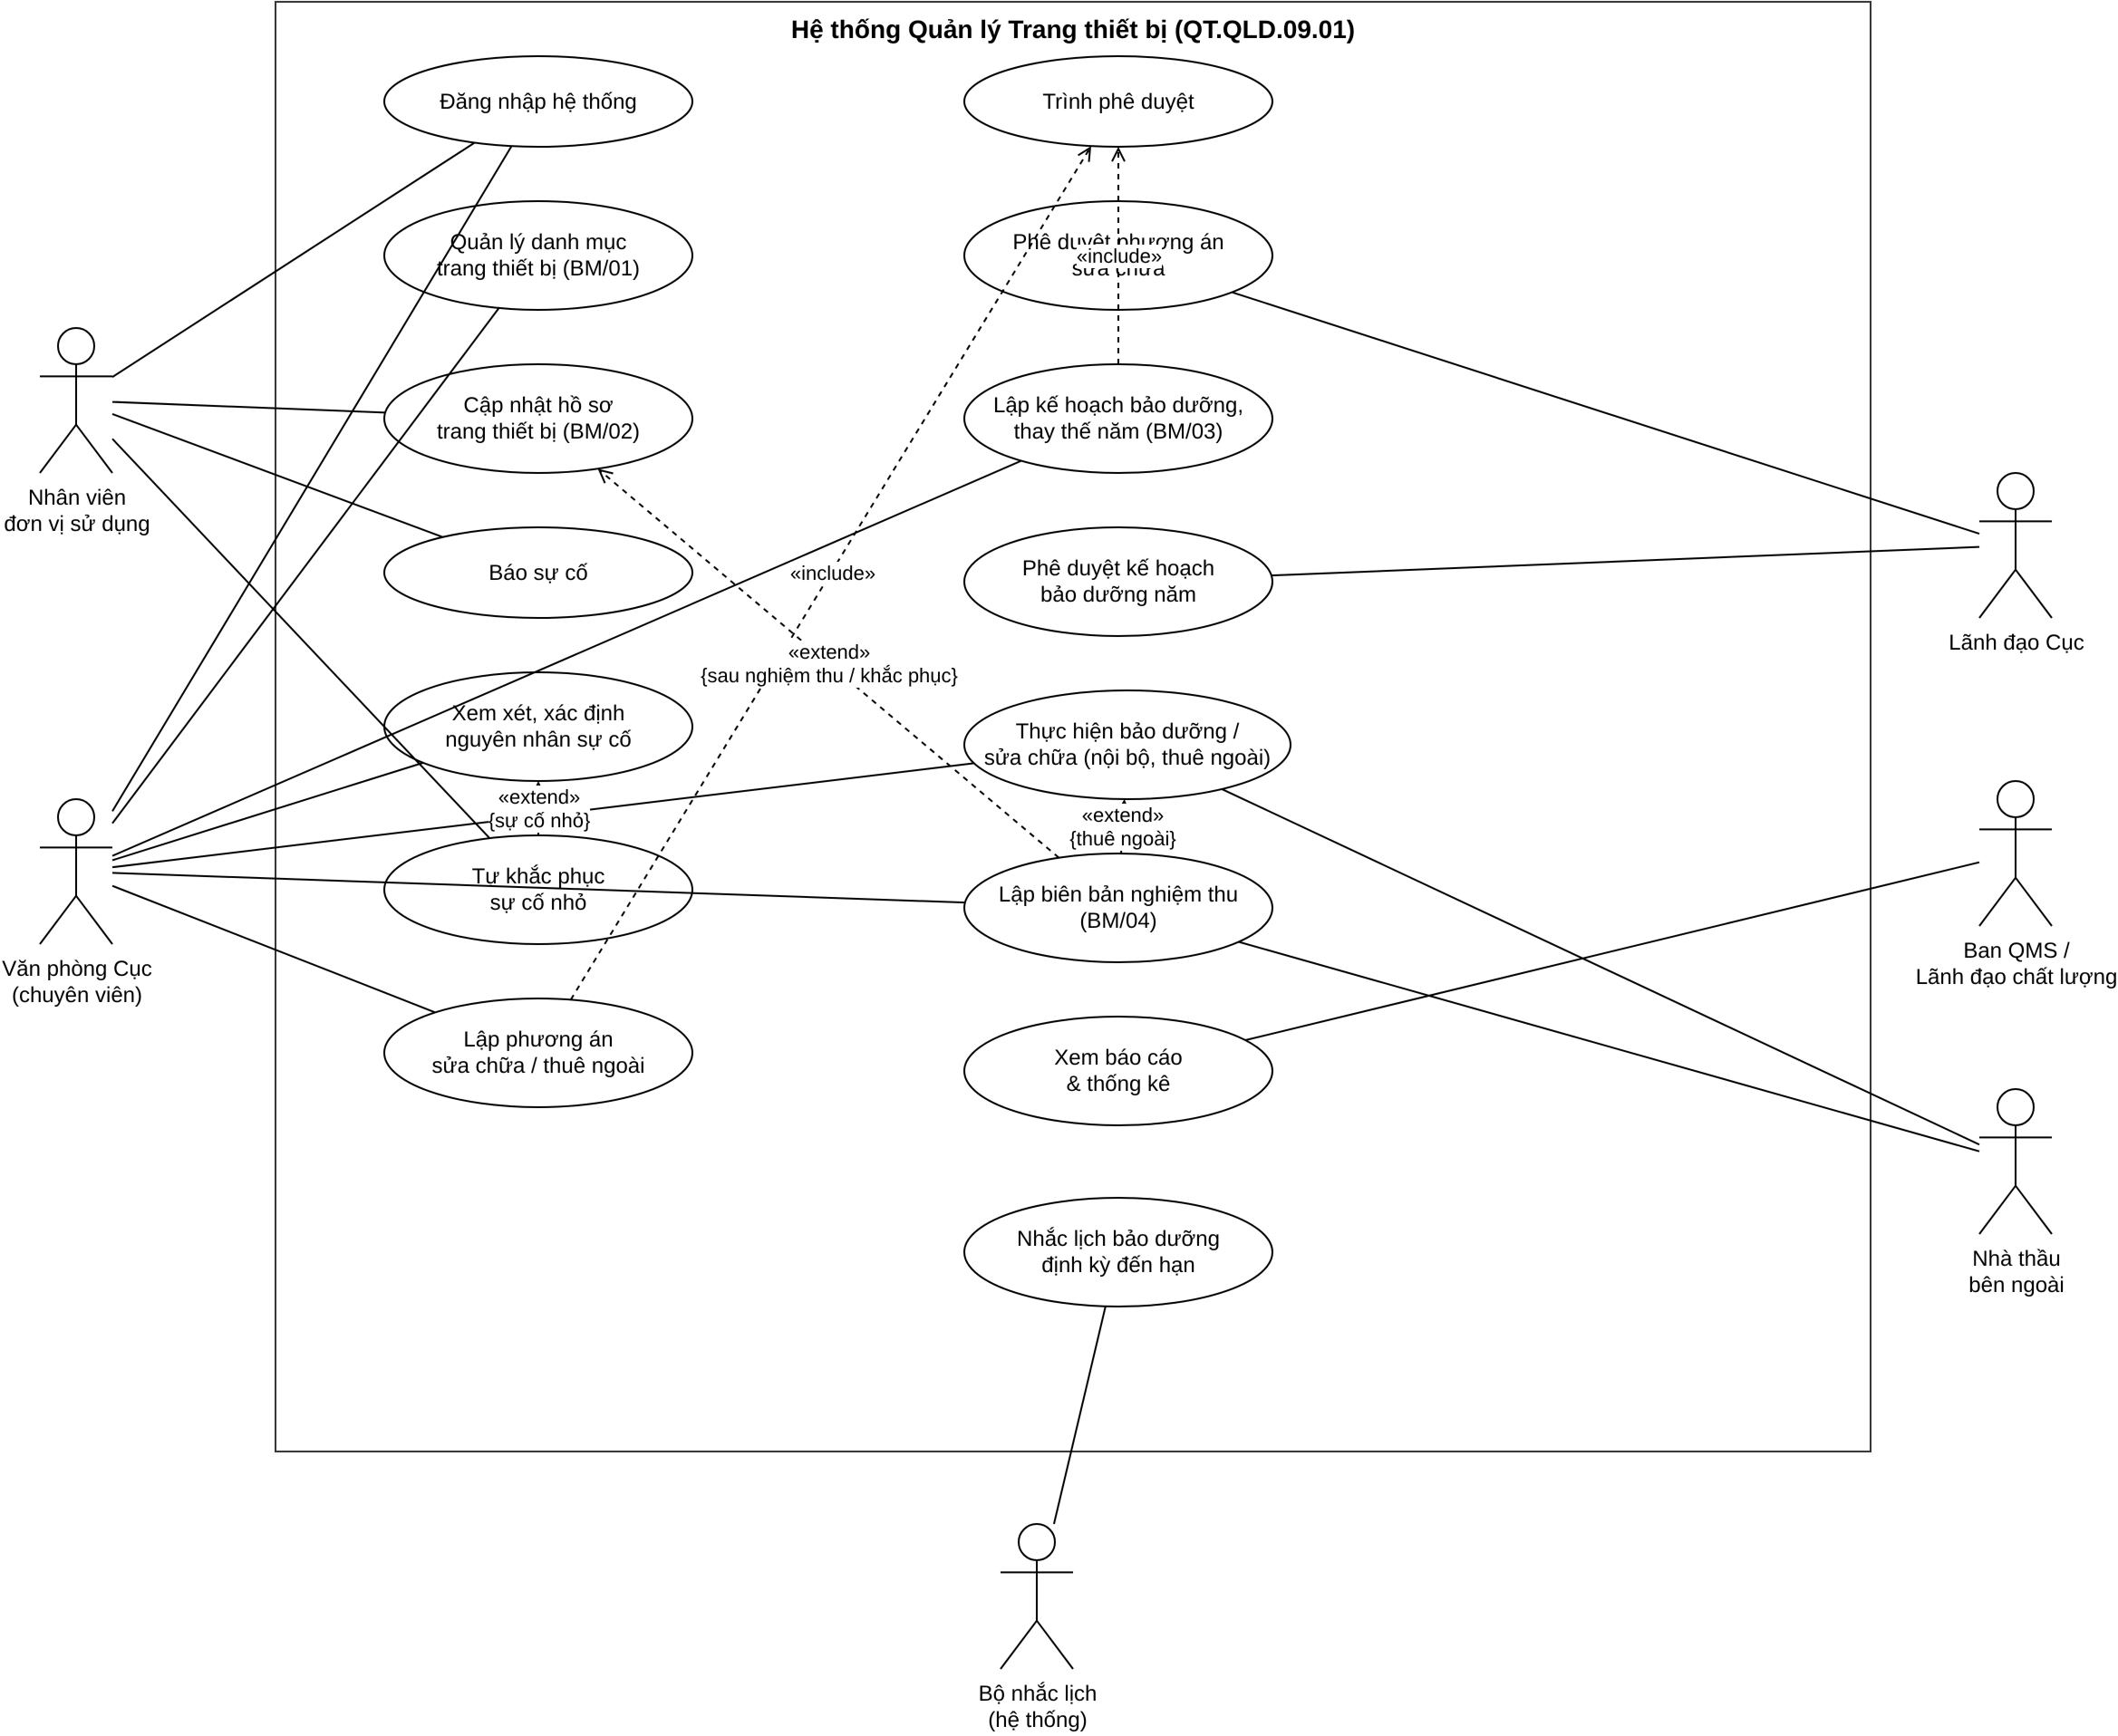
\includegraphics[width=\textwidth]{figures/use-case.png}}{\fbox{\parbox{0.9\textwidth}{\centering Sơ đồ use case (xem file \texttt{docs/diagrams/01-use-case.drawio} — mở bằng draw.io)}}}
\caption{Sơ đồ use case tổng quát của hệ thống}
\label{fig:usecase}
\end{figure}

\section{Đặc tả use case chính}

\begin{table}[h]
\centering
\caption{Đặc tả UC-04: Báo sự cố}
\label{tab:uc04}
\begin{tabular}{P{3.2cm}P{11.8cm}}
\toprule
\textbf{Use case} & UC-04 — Báo sự cố \\
\textbf{Tác nhân} & Nhân viên đơn vị sử dụng (chính); Văn phòng Cục (bổ sung) \\
\textbf{Tiền điều kiện} & Đã đăng nhập (UC-01); thiết bị nằm trong danh mục và thuộc đơn vị \\
\textbf{Hậu điều kiện} & Sự cố tạo mới với trạng thái ``Mới''; thiết bị chuyển ``Sự cố''; Văn phòng Cục nhận thông báo \\
\midrule
\textbf{Luồng chính} & 1. Đơn vị chọn ``Báo sự cố''. \; 2. Hệ thống hiển thị danh sách thiết bị của đơn vị. \; 3. Đơn vị chọn thiết bị, chọn mức độ ước lượng (nhỏ/nguy cơ/lớn), nhập mô tả. \; 4. Hệ thống kiểm tra dữ liệu hợp lệ. \; 5. Hệ thống sinh mã sự cố (SC-<năm>-<số thứ tự>), lưu với trạng thái ``Mới'', chuyển thiết bị sang ``Sự cố'', gửi thông báo cho Văn phòng Cục, ghi audit log. \; 6. Hệ thống hiển thị mã sự cố cho đơn vị. \\
\textbf{Luồng thay thế} & 4a. Thiếu thiết bị/mô tả: hiển thị lỗi, quay lại bước 3. \newline 5a. Thiết bị không tồn tại hoặc không thuộc đơn vị: báo lỗi 404/403. \\
\bottomrule
\end{tabular}
\end{table}

\begin{table}[h]
\centering
\caption{Đặc tả UC-05 + UC-06: Xem xét nguyên nhân và tự khắc phục}
\label{tab:uc05}
\begin{tabular}{P{3.2cm}P{11.8cm}}
\toprule
\textbf{Use case} & UC-05 — Xem xét, xác định nguyên nhân (gồm UC-06) \\
\textbf{Tác nhân} & Văn phòng Cục (chính), Đơn vị (trong UC-06) \\
\textbf{Tiền điều kiện} & Tồn tại sự cố trạng thái ``Mới'' \\
\textbf{Hậu điều kiện} & Nếu [nhỏ]: sự cố ở ``Đang xem xét'' với phân loại ``Tự khắc phục''; nếu [lớn]: ``Chờ phê duyệt'' chờ lập phương án \\
\midrule
\textbf{Luồng chính} & 1. Văn phòng Cục mở danh sách sự cố ``Mới''. \; 2. Chọn ``Xem xét'', nhập mức độ, nguyên nhân. \; 3. Chọn phân loại: \emph{Tự khắc phục} / \emph{Nội bộ} / \emph{Thuê ngoài}. \; 4. Hệ thống cập nhật trạng thái: [tự khắc phục] $\rightarrow$ ``Đang xem xét'' và thông báo cho đơn vị; [khác] $\rightarrow$ ``Chờ phê duyệt''. \; 5. Ghi audit log. \\
\textbf{UC-06} & 6. Đơn vị mở ``Sự cố của đơn vị'', chọn ``Tự khắc phục'', nhập nội dung khắc phục. \; 7. Hệ thống \textbf{tự động ghi một bản ghi vào hồ sơ thiết bị (BM/02)}, đóng sự cố, trả thiết bị về ``Hoạt động''. \; \textbf{Không có bước phê duyệt} — đúng mục 6.2.3b. \\
\textbf{Luồng thay thế} & 7a. Thiếu nội dung khắc phục: báo lỗi, giữ trạng thái. \newline 2a. Sự cố không ở trạng thái ``Mới'': từ chối (409). \\
\bottomrule
\end{tabular}
\end{table}

\begin{table}[h]
\centering
\caption{Đặc tả UC-10 + UC-11: Lập và phê duyệt kế hoạch bảo dưỡng năm}
\label{tab:uc10}
\begin{tabular}{P{3.2cm}P{11.8cm}}
\toprule
\textbf{Use case} & UC-10 — Lập kế hoạch bảo dưỡng, thay thế năm (gồm UC-11) \\
\textbf{Tác nhân} & Văn phòng Cục (chính); Lãnh đạo Cục (UC-11) \\
\textbf{Tiền điều kiện} & Đã có danh mục thiết bị; chưa tồn tại kế hoạch của năm đó \\
\textbf{Hậu điều kiện} & Kế hoạch ở trạng thái ``Nháp'' (chưa trình) hoặc ``Đã duyệt'' \\
\midrule
\textbf{Luồng chính} & 1. Văn phòng Cục chọn ``Lập kế hoạch'', nhập năm. \; 2. Thêm từng hạng mục: thiết bị + nội dung + đơn vị thực hiện (nội bộ/bên ngoài) + tháng dự kiến (+ chi phí, ưu tiên — mở rộng). \; 3. Hệ thống tạo kế hoạch ``Nháp'' với các hạng mục ``Chờ thực hiện''. \; 4. Bấm ``Trình Lãnh đạo Cục'' $\rightarrow$ trạng thái ``Chờ duyệt'' + thông báo cho Lãnh đạo Cục. \; 5. Lãnh đạo Cục xem, bấm ``Phê duyệt'' $\rightarrow$ ``Đã duyệt'' + thông báo cho Văn phòng Cục; hoặc ``Trả về'' kèm lý do $\rightarrow$ ``Từ chối'' (quay lại bước 2 để sửa). \\
\textbf{Luồng thay thế} & 3a. Năm kế hoạch đã tồn tại: báo lỗi 409. \newline 5a. Từ chối không ghi lý do: hệ thống bắt buộc nhập lý do. \\
\bottomrule
\end{tabular}
\end{table}

\begin{table}[h]
\centering
\caption{Đặc tả UC-13: Lập biên bản nghiệm thu và ký duyệt}
\label{tab:uc13}
\begin{tabular}{P{3.2cm}P{11.8cm}}
\toprule
\textbf{Use case} & UC-13 — Lập biên bản nghiệm thu (BM/04) \\
\textbf{Tác nhân} & Văn phòng Cục (lập); Lãnh đạo Cục / Đơn vị / Nhà thầu (ký) \\
\textbf{Tiền điều kiện} & Phương án sửa chữa đã hoàn thành (sự cố ``Chờ nghiệm thu''), hoặc hạng mục bảo dưỡng cần nghiệm thu \\
\textbf{Hậu điều kiện} & Đủ chữ ký: sự cố đóng, hồ sơ thiết bị thêm bản ghi ``Sửa chữa'', thiết bị về ``Hoạt động'' \\
\midrule
\textbf{Luồng chính} & 1. Văn phòng Cục chọn phương án đã hoàn thành, bấm ``Lập biên bản''. \; 2. Nhập ``Bên B đã thực hiện...'', ``Tình trạng hoạt động sau khi Bên B thực hiện...'', ngày lập; nhập đại diện Bên A (tối thiểu 1) và Bên B (tối thiểu 1) — đúng cấu trúc BM/04 (hệ thống ghi ``lập thành 02 bản''). \; 3. Hệ thống sinh mã BBNT-<năm>-<STT>, lưu biên bản ``Mới''. \; 4. Các đại diện ký (mô phỏng chữ ký số). \; 5. Khi đủ chữ ký: hệ thống ghi hồ sơ thiết bị, đóng sự cố, trả thiết bị về ``Hoạt động'', đánh dấu biên bản ``Đã ký''. \\
\textbf{Luồng thay thế} & 2a. Thiếu đại diện một trong hai bên: từ chối tạo. \newline 4a. Chưa đủ chữ ký: giữ ``Mới'', hiển thị tiến độ ký n/m. \\
\bottomrule
\end{tabular}
\end{table}

\section{Sơ đồ hoạt động (Activity Diagram)}

\begin{figure}[h]
\centering
\IfFileExists{figures/activity-incident.png}{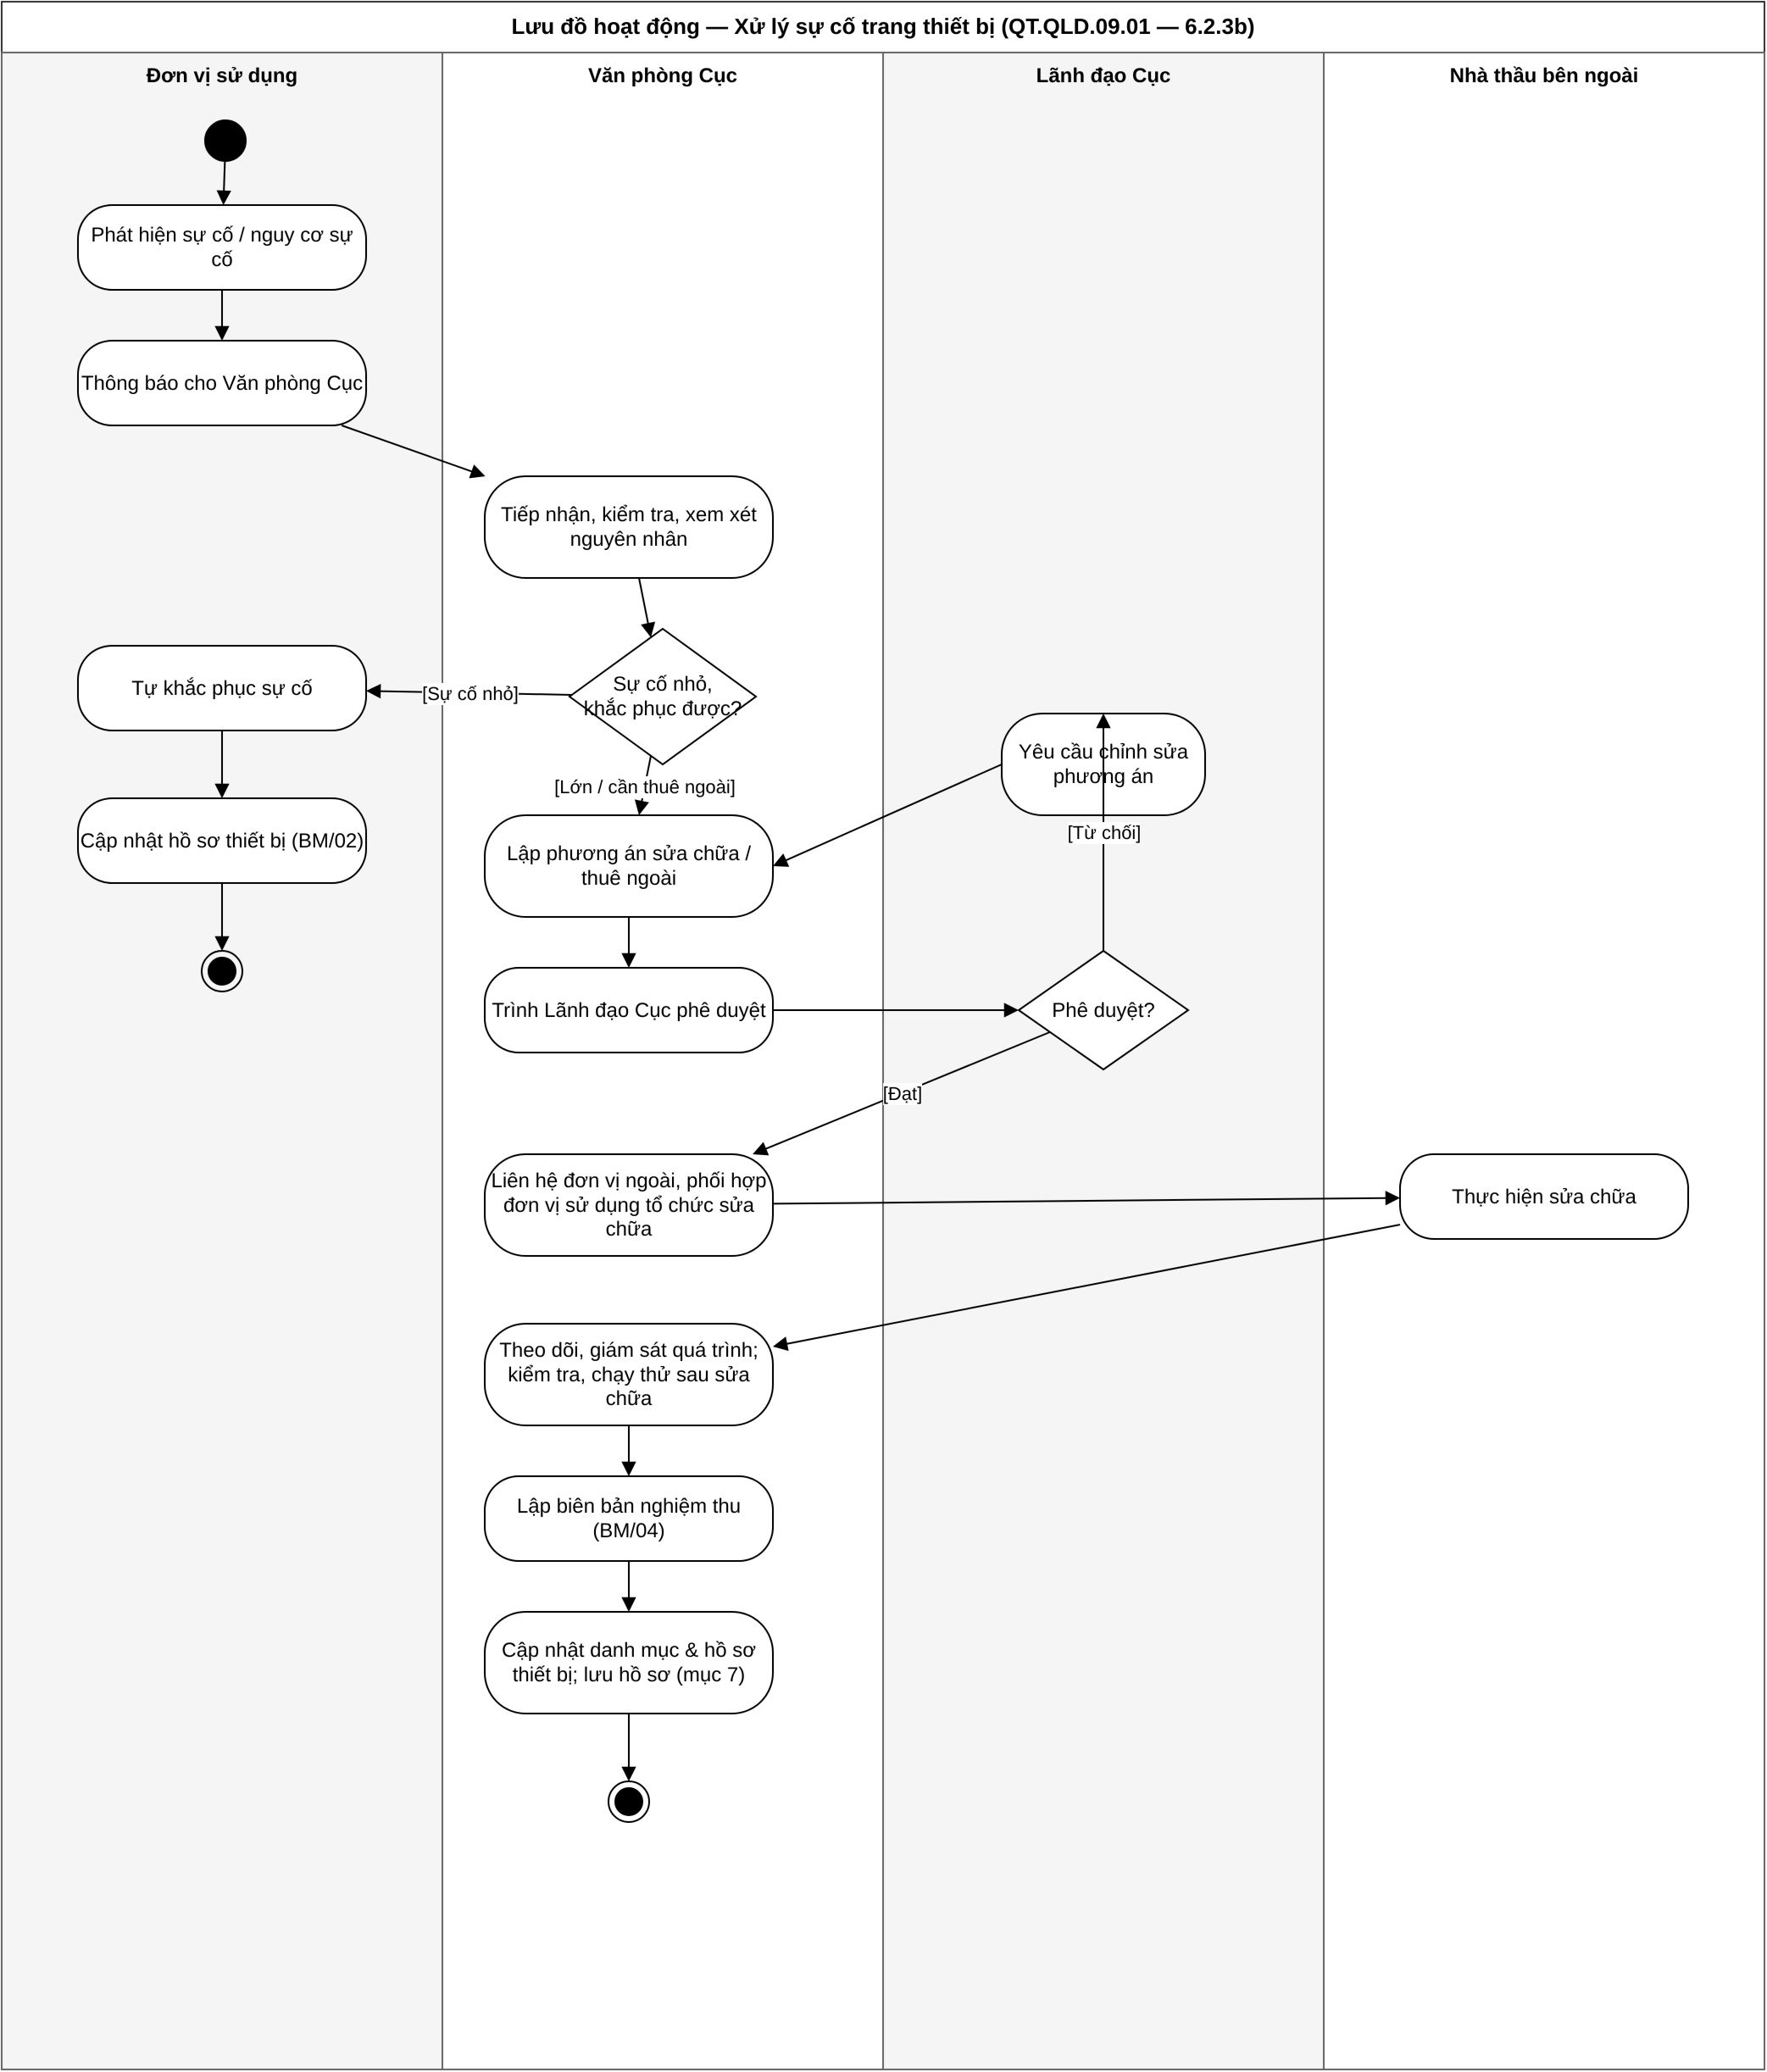
\includegraphics[width=0.86\textwidth]{figures/activity-incident.png}}{\fbox{\parbox{0.9\textwidth}{\centering Sơ đồ hoạt động xử lý sự cố (file \texttt{docs/diagrams/02-activity.drawio}, trang 1)}}}
\caption{Sơ đồ hoạt động — xử lý sự cố (4 phân làn: Đơn vị, Văn phòng Cục, Lãnh đạo Cục, Nhà thầu)}
\label{fig:act-incident}
\end{figure}

Sơ đồ Hình~\ref{fig:act-incident} thể hiện đúng điểm quyết định của mục 6.2.3b: sau khi Văn phòng Cục ``kiểm tra, xem xét nguyên nhân'', nhánh \textbf{[Sự cố nhỏ]} đi thẳng sang làn Đơn vị (tự khắc phục $\rightarrow$ cập nhật hồ sơ $\rightarrow$ kết thúc); nhánh \textbf{[Lớn/cần thuê ngoài]} phải qua làn Lãnh đạo Cục (phê duyệt), nếu bị từ chối quay lại lập lại phương án.

\begin{figure}[h]
\centering
\IfFileExists{figures/activity-plan.png}{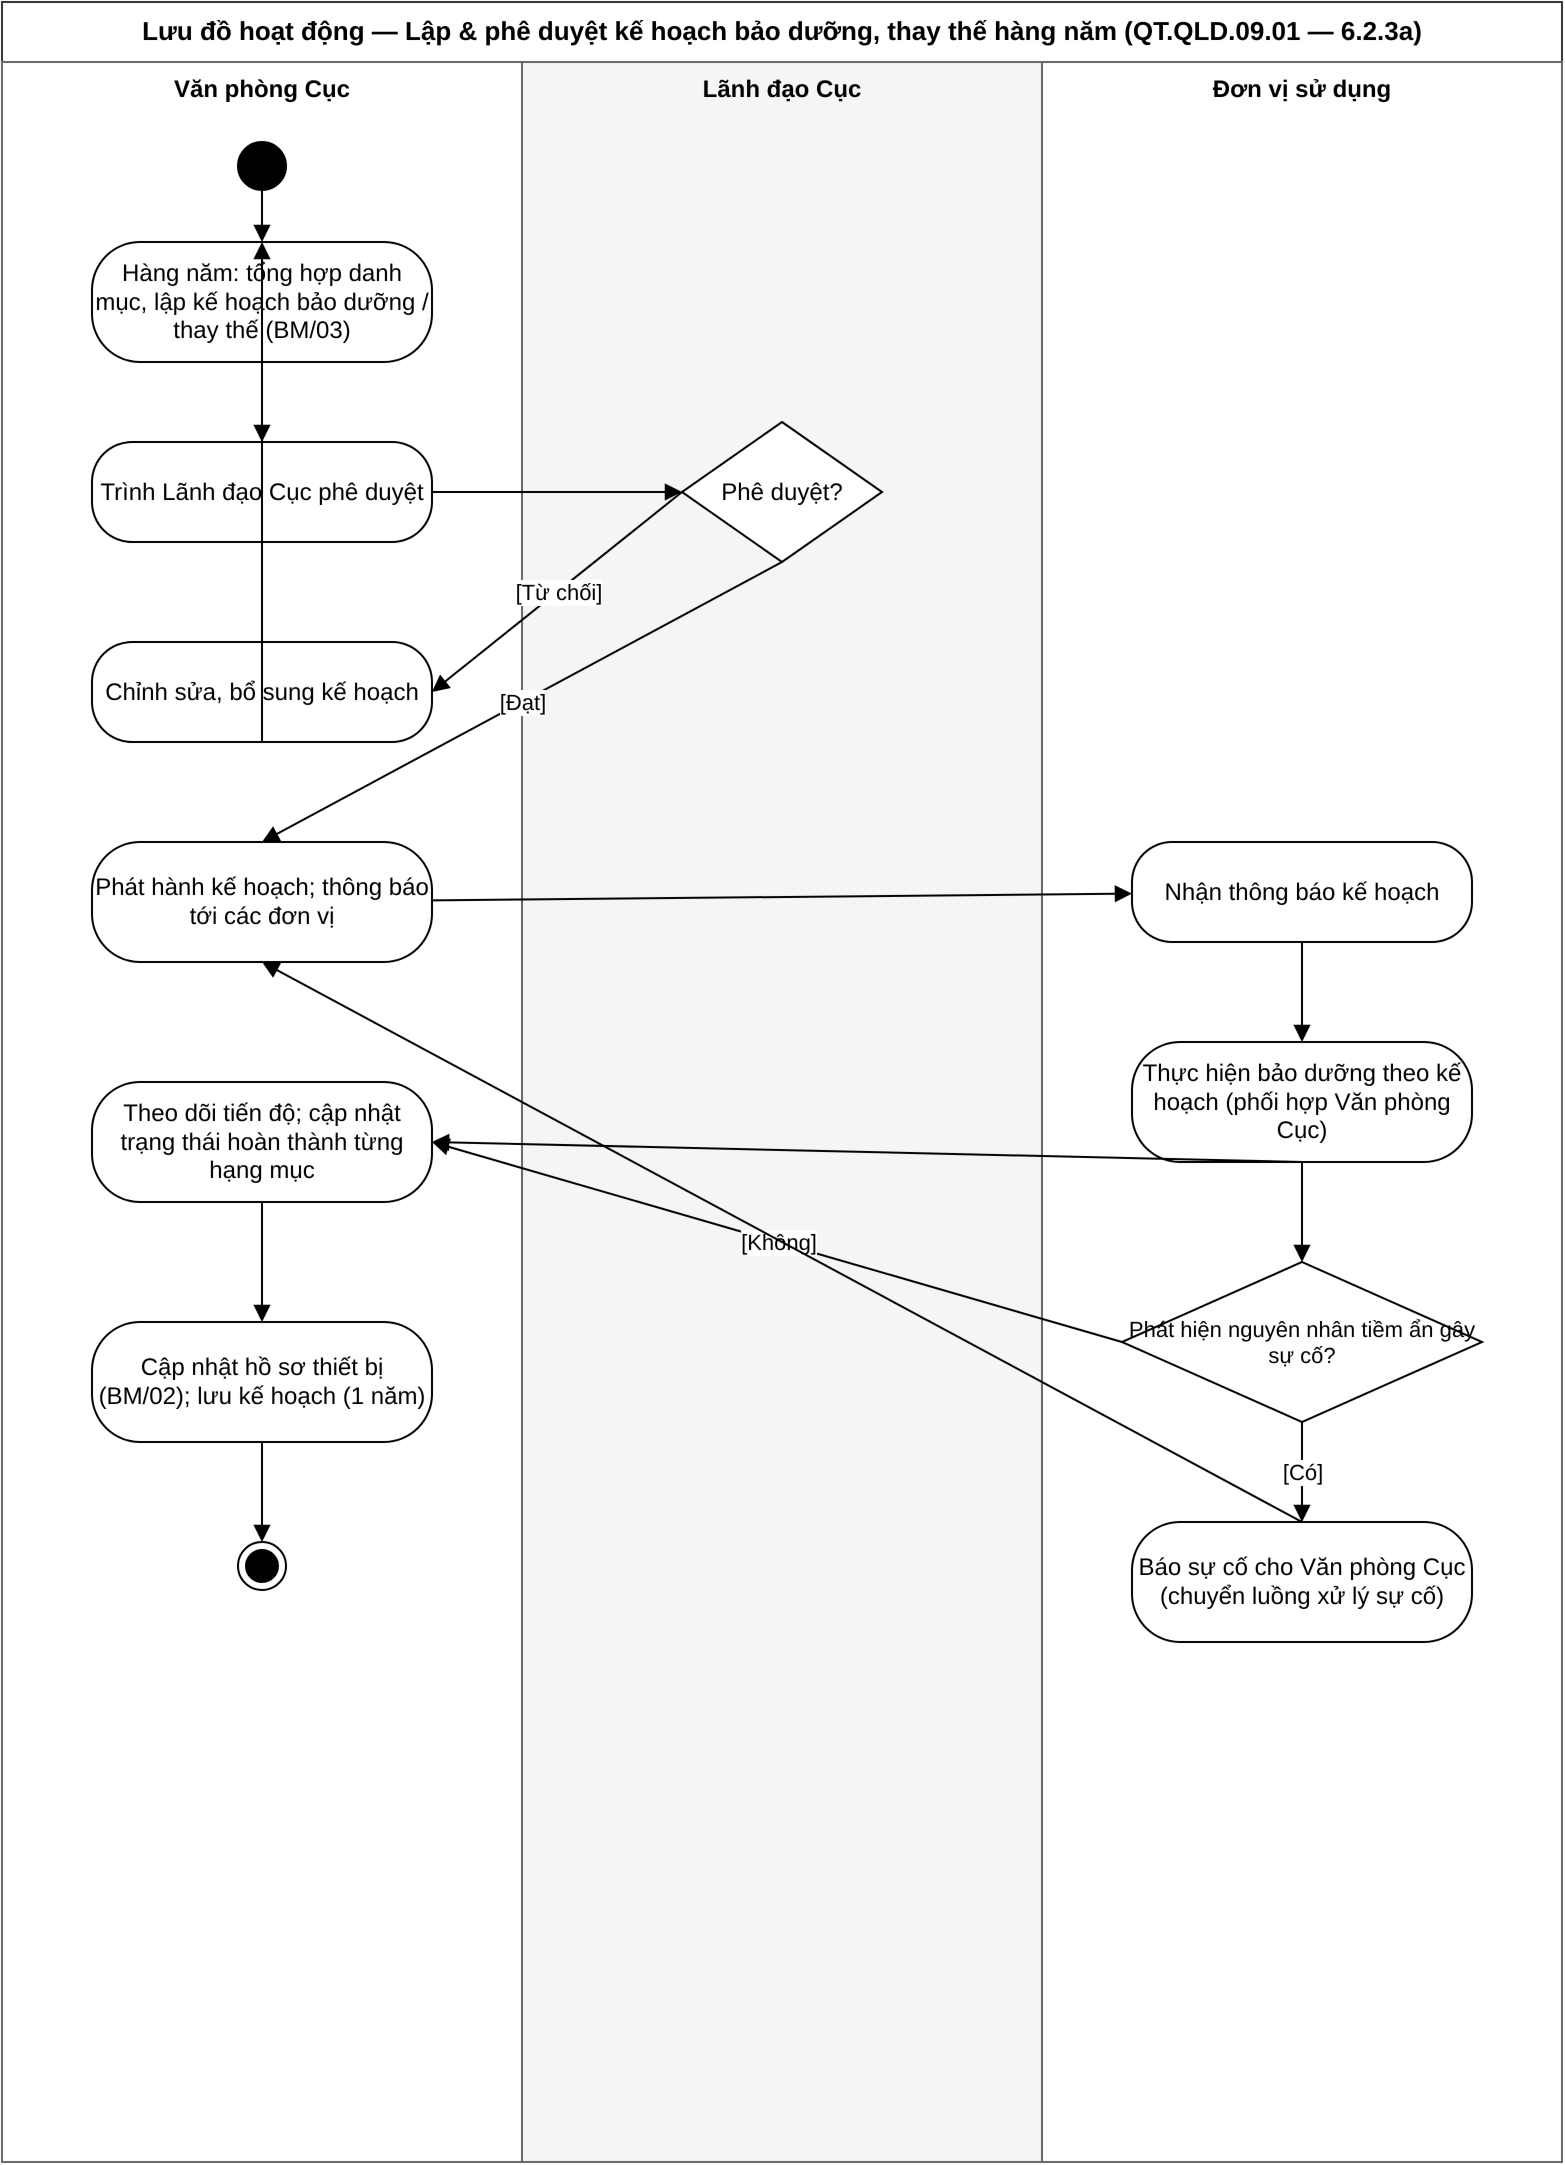
\includegraphics[width=0.8\textwidth]{figures/activity-plan.png}}{\fbox{\parbox{0.9\textwidth}{\centering Sơ đồ hoạt động kế hoạch bảo dưỡng (file \texttt{docs/diagrams/02-activity.drawio}, trang 2)}}}
\caption{Sơ đồ hoạt động — lập và phê duyệt kế hoạch bảo dưỡng hàng năm}
\label{fig:act-plan}
\end{figure}

Sơ đồ Hình~\ref{fig:act-plan} mô tả luồng kế hoạch hàng năm: vòng lặp ``từ chối — chỉnh sửa'' giữa Văn phòng Cục và Lãnh đạo Cục, sau khi phát hành thì các đơn vị thực hiện; nếu phát hiện nguyên nhân tiềm tàng gây sự cố thì chuyển sang luồng xử lý sự cố (mục 6.2.4).

\chapter{Mô hình hóa cấu trúc}

\section{Phương pháp xác định lớp}

Áp dụng kỹ thuật \textbf{phân tích danh từ} (noun analysis) trên bốn biểu mẫu và mô tả quy trình (Chương 2), nhóm rút ra các danh từ ứng viên rồi loại bỏ: (i) danh từ trùng lặp/đồng nghĩa, (ii) thuộc tính thực chất là thuộc tính, (iii) danh từ ngoài phạm vi. Kết quả: 15 lớp doanh nghiệp.

\begin{table}[h]
\centering
\caption{Danh sách lớp doanh nghiệp và trách nhiệm}
\label{tab:classes}
\begin{tabular}{P{3.4cm}P{12cm}}
\toprule
\textbf{Lớp} & \textbf{Trách nhiệm} \\
\midrule
NguoiDung & Tài khoản người dùng: đăng nhập, thông tin cá nhân, thuộc một vai trò và (tùy chọn) một đơn vị \\
VaiTro & Định nghĩa vai trò phân quyền: DON\_VI, VAN\_PHONG\_CUC, LANH\_DAO\_CUC, QMS, NHA\_THAU \\
DonVi & Đơn vị/phòng thuộc Cục sử dụng thiết bị \\
TrangThietBi & Thiết bị: thuộc tính đúng BM/01 (mã số, tên, nước sản xuất, ngày nhận, đơn vị); trạng thái vòng đời; kiểm tra nhắc bảo dưỡng \\
HoSoThietBi & Một bản ghi lịch sử của thiết bị — đúng bảng BM/02 (ngày thực hiện, nội dung, người thực hiện); chỉ thêm, không sửa/xóa \\
KeHoachBaoDuong & Kế hoạch năm (BM/03 — header): năm, trạng thái phê duyệt, người duyệt \\
ChiTietKeHoach & Hạng mục kế hoạch (BM/03 — dòng): nội dung, đơn vị thực hiện (nội bộ/bên ngoài), tháng dự kiến, ghi chú; trạng thái tiến độ \\
SuCo & Sự cố: mã, mô tả, mức độ, phân loại xử lý, trạng thái theo vòng đời xử lý \\
PhuongAnSuaChua & Phương án sửa chữa/thuê ngoài: nội dung, chi phí dự kiến, trạng thái phê duyệt \\
NhaThau & Nhà cung cấp dịch vụ bảo dưỡng/sửa chữa ngoài (mở rộng) \\
BienBanNghiemThu & Biên bản nghiệm thu (BM/04): nội dung đã thực hiện, tình trạng sau thực hiện, ngày lập, số bản (02) \\
DaiDien & Người đại diện hai bên trong biên bản: bên (A/B), họ tên, đơn vị, đã ký \\
TaiLieuDinhKem & File đính kèm đa hình: gắn vào thiết bị/sự cố/nghiệm thu/kế hoạch \\
ThongBao & Thông báo trong hệ thống (nhắc lịch, phê duyệt, sự cố) \\
NhatKyHeThong & Audit trail append-only: hành động, đối tượng, dữ liệu cũ/mới (ISO 9001) \\
\bottomrule
\end{tabular}
\end{table}

\section{Thẻ CRC}

\begin{table}[h]
\centering
\begin{tabular}{|P{5.2cm}|P{5.2cm}|}
\hline
\multicolumn{2}{|l|}{\textbf{Lớp: TrangThietBi}} \\
\hline
\textbf{Trách nhiệm (Responsibilities)} & \textbf{Cộng tác viên (Collaborators)} \\
\hline
Giữ thông tin nhận dạng thiết bị (BM/01) \newline Quản lý trạng thái vòng đời \newline Cung cấp lịch sử hồ sơ \newline Kiểm tra hạng mục bảo dưỡng đến hạn & HoSoThietBi (tạo bản ghi) \newline DonVi (thuộc đơn vị) \newline SuCo (gắn sự cố) \newline ChiTietKeHoach (gắn kế hoạch) \\
\hline
\end{tabular}
\end{table}

\begin{table}[h]
\centering
\begin{tabular}{|P{5.2cm}|P{5.2cm}|}
\hline
\multicolumn{2}{|l|}{\textbf{Lớp: SuCo}} \\
\hline
\textbf{Trách nhiệm} & \textbf{Cộng tác viên} \\
\hline
Tiếp nhận báo sự cố \newline Chuyển trạng thái xử lý \newline Định tuyến: tự khắc phục / lập phương án \newline Đóng sự cố sau nghiệm thu & TrangThietBi (thiết bị hỏng) \newline NguoiDung (người báo, người xem xét) \newline PhuongAnSuaChua (tạo khi thuê ngoài) \newline BienBanNghiemThu (đóng khi đủ chữ ký) \\
\hline
\end{tabular}
\end{table}

\begin{table}[h]
\centering
\begin{tabular}{|P{5.2cm}|P{5.2cm}|}
\hline
\multicolumn{2}{|l|}{\textbf{Lớp: BienBanNghiemThu}} \\
\hline
\textbf{Trách nhiệm} & \textbf{Cộng tác viên} \\
\hline
Ghi nhận nội dung đã thực hiện và tình trạng sau thực hiện (BM/04) \newline Quản lý danh sách đại diện hai bên \newline Ghi hồ sơ thiết bị khi đủ chữ ký & DaiDien (hợp thành 2--4) \newline PhuongAnSuaChua (nguồn nghiệm thu) \newline HoSoThietBi (tự tạo bản ghi) \newline SuCo (đóng sự cố) \\
\hline
\end{tabular}
\end{table}

\section{Sơ đồ lớp}

\begin{figure}[h]
\centering
\IfFileExists{figures/class.png}{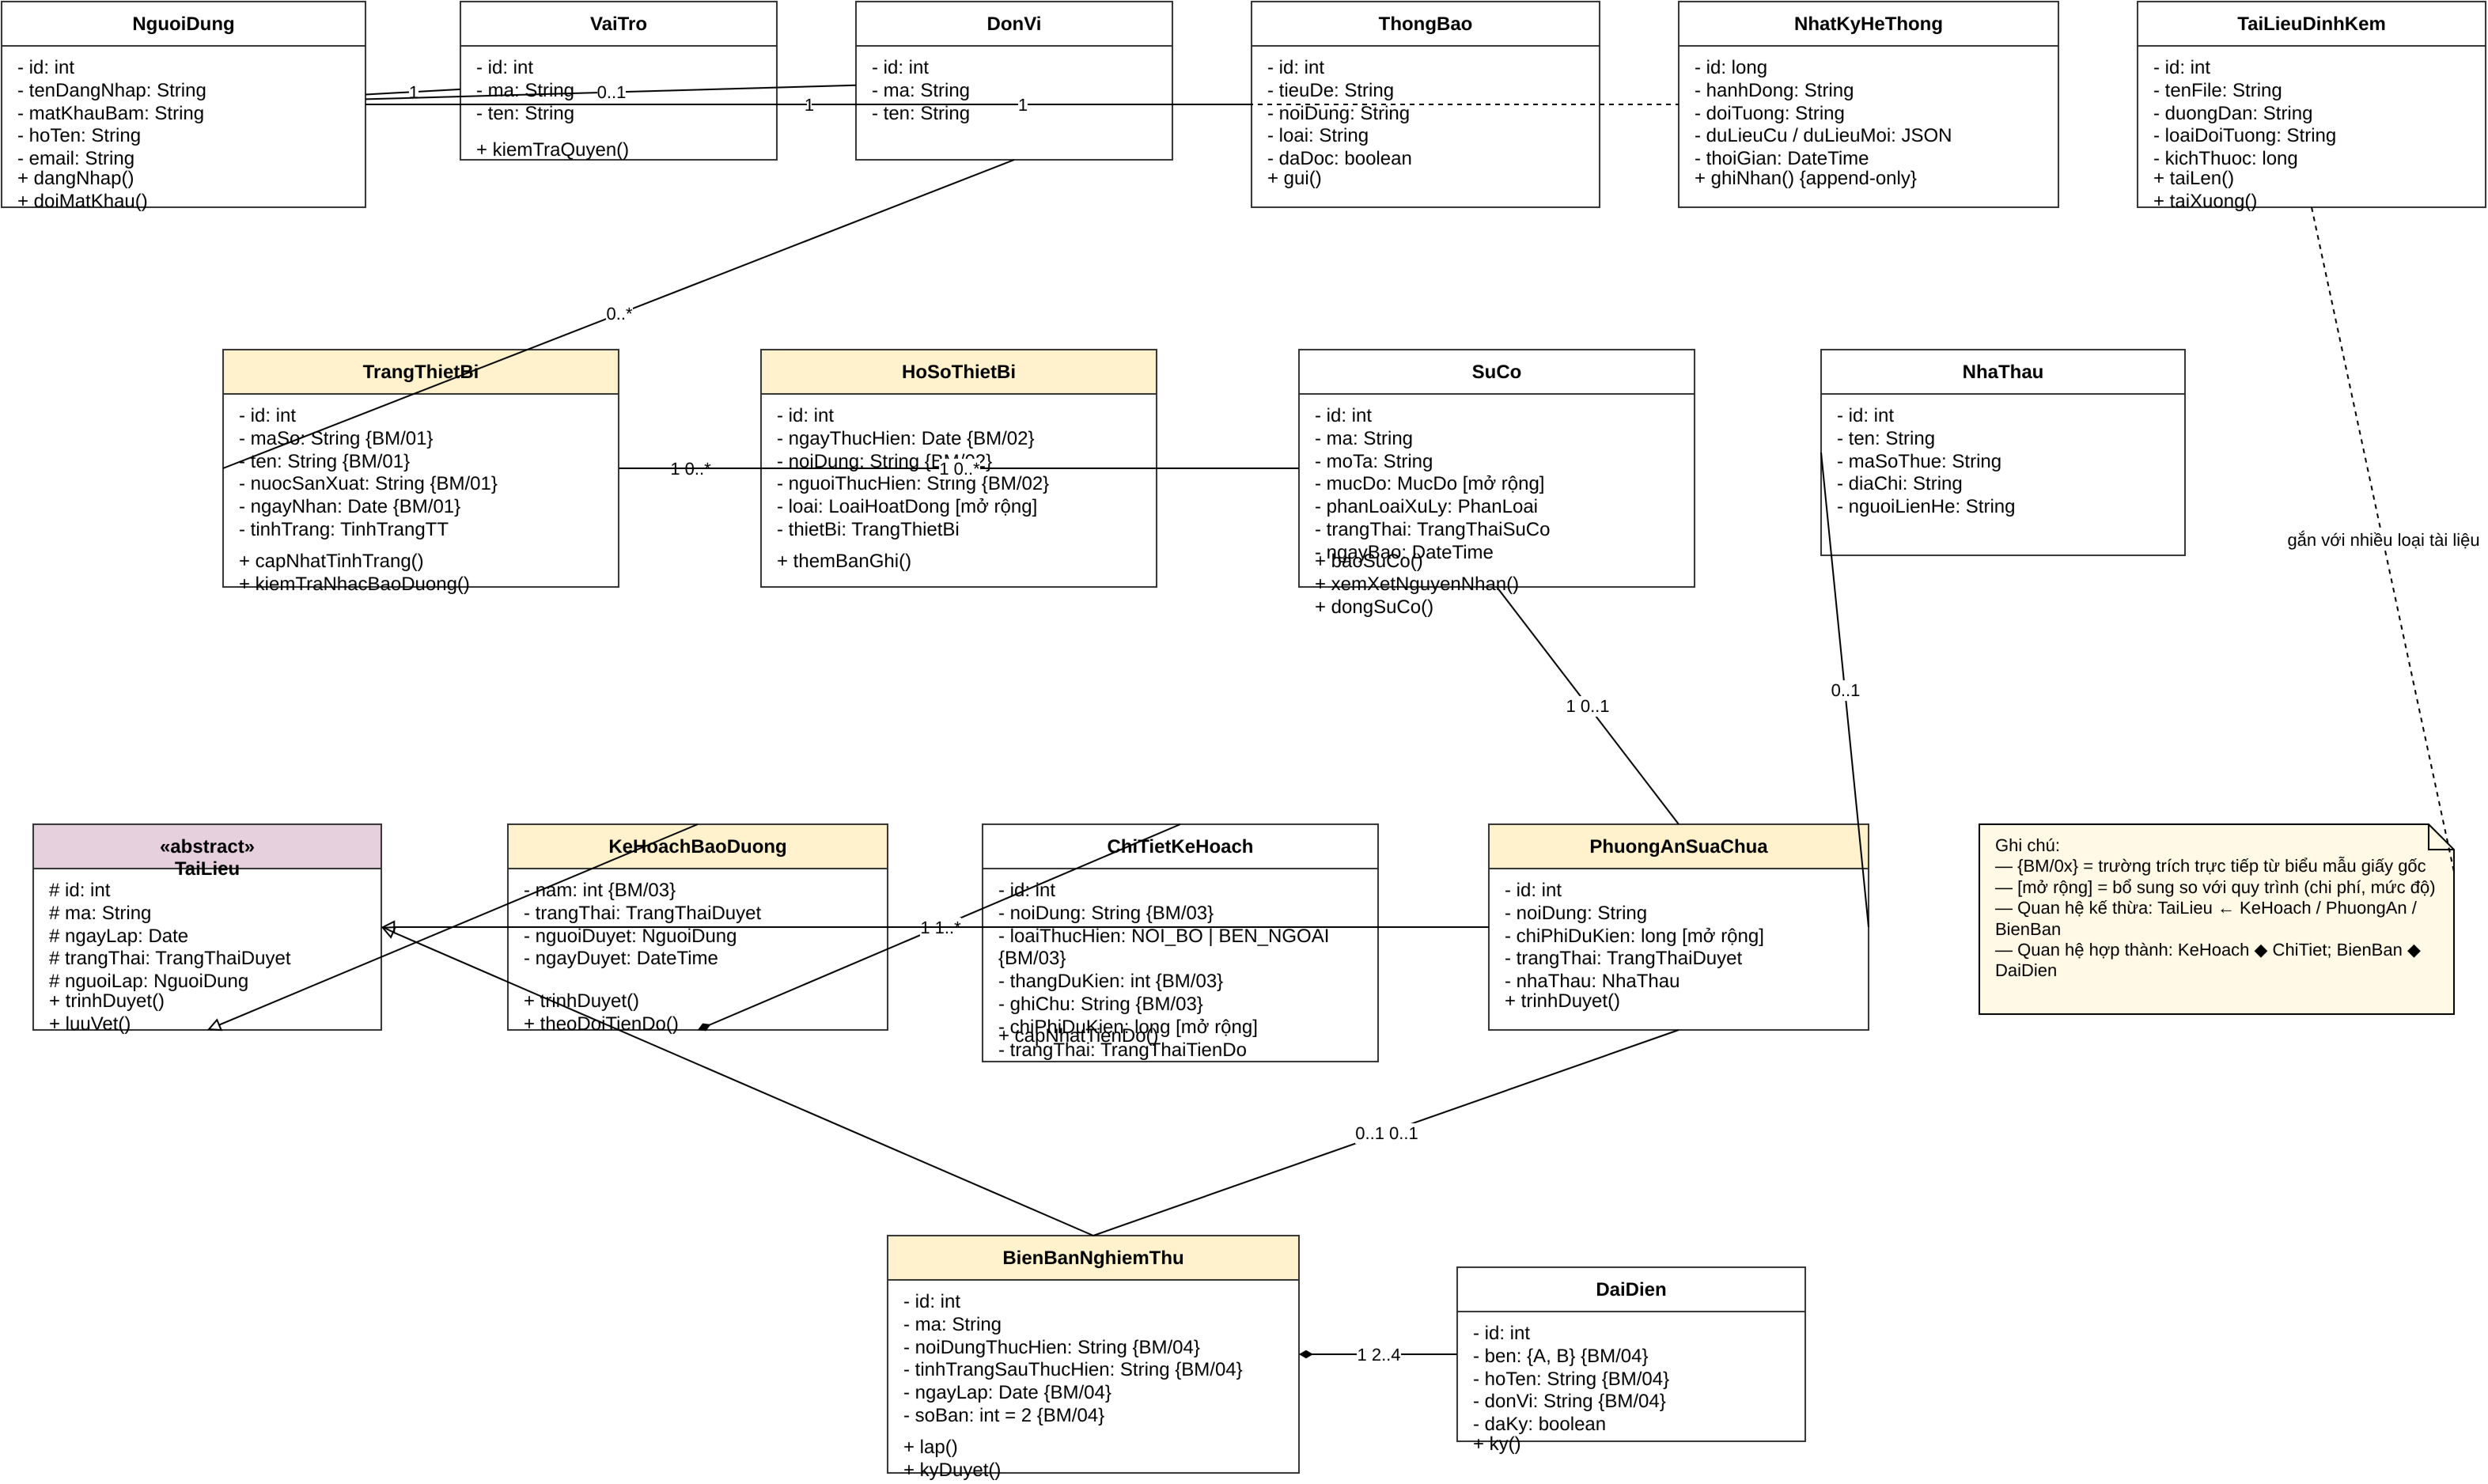
\includegraphics[width=\textwidth]{figures/class.png}}{\fbox{\parbox{0.9\textwidth}{\centering Sơ đồ lớp (file \texttt{docs/diagrams/03-class.drawio})}}}
\caption{Sơ đồ lớp của hệ thống}
\label{fig:class}
\end{figure}

\subsection{Các quan hệ chính}

\begin{itemize}
  \item \textbf{Kết tập/gắn kết một--nhiều:} TrangThietBi 1 --- 0..* HoSoThietBi; TrangThietBi 1 --- 0..* SuCo; SuCo 1 --- 0..1 PhuongAnSuaChua; PhuongAnSuaChua 0..1 --- 0..1 BienBanNghiemThu; ChiTietKeHoach * --- 1 TrangThietBi.
  \item \textbf{Hợp thành (composition):}
  \begin{itemize}
    \item \emph{KeHoachBaoDuong $\blacklozenge$--- 1..* ChiTietKeHoach}: hạng mục không tồn tại độc lập ngoài kế hoạch; xóa kế hoạch thì xóa hạng mục.
    \item \emph{BienBanNghiemThu $\blacklozenge$--- 2..4 DaiDien}: đại diện là cấu phần bắt buộc của biên bản (Bên A + Bên B, mỗi bên 1--2 người), đúng cấu trúc BM/04.
  \end{itemize}
  \item \textbf{Kế thừa (generalization):} lớp trừu tượng \emph{TaiLieu} (mã, ngày lập, trạng thái phê duyệt, người lập; hành vi \texttt{trinhDuyet()}, \texttt{luuVet()}) là lớp cha của \emph{KeHoachBaoDuong}, \emph{PhuongAnSuaChua}, \emph{BienBanNghiemThu} — ba loại ``tài liệu'' đều đi qua vòng đời trình duyệt và cần lưu vết.
  \item \textbf{Phân quyền:} NguoiDung * --- 1 VaiTro; NguoiDung * --- 0..1 DonVi.
  \item Trong sơ đồ, trường mang nhãn \{BM/0x\} trích trực tiếp từ biểu mẫu giấy; nhãn [mở rộng] là bổ sung đề xuất (chi phí, mức độ ưu tiên) — tách bạch với nguyên bản.
\end{itemize}

\subsection{Ánh xạ lớp $\rightarrow$ bảng dữ liệu}

Sơ đồ lớp được ánh xạ 1--1 sang lược đồ quan hệ PostgreSQL (chi tiết đầy đủ ở Chương 6): mỗi lớp một bảng; quan hệ nhiều--một qua khóa ngoại; hợp thành qua ràng buộc \texttt{ON DELETE CASCADE}; kế thừa TaiLieu được ``phẳng hóa'' (các thuộc tính chung lặp lại trong từng bảng con) vì số lượng lớp con ít và giúp truy vấn đơn giản — quyết định được cân nhắc trong thiết kế.

\chapter{Mô hình hóa hành vi}

\section{Sơ đồ trình tự}

\subsection{Xử lý sự cố (nhánh thuê ngoài)}

\begin{figure}[h]
\centering
\IfFileExists{figures/sequence-incident.png}{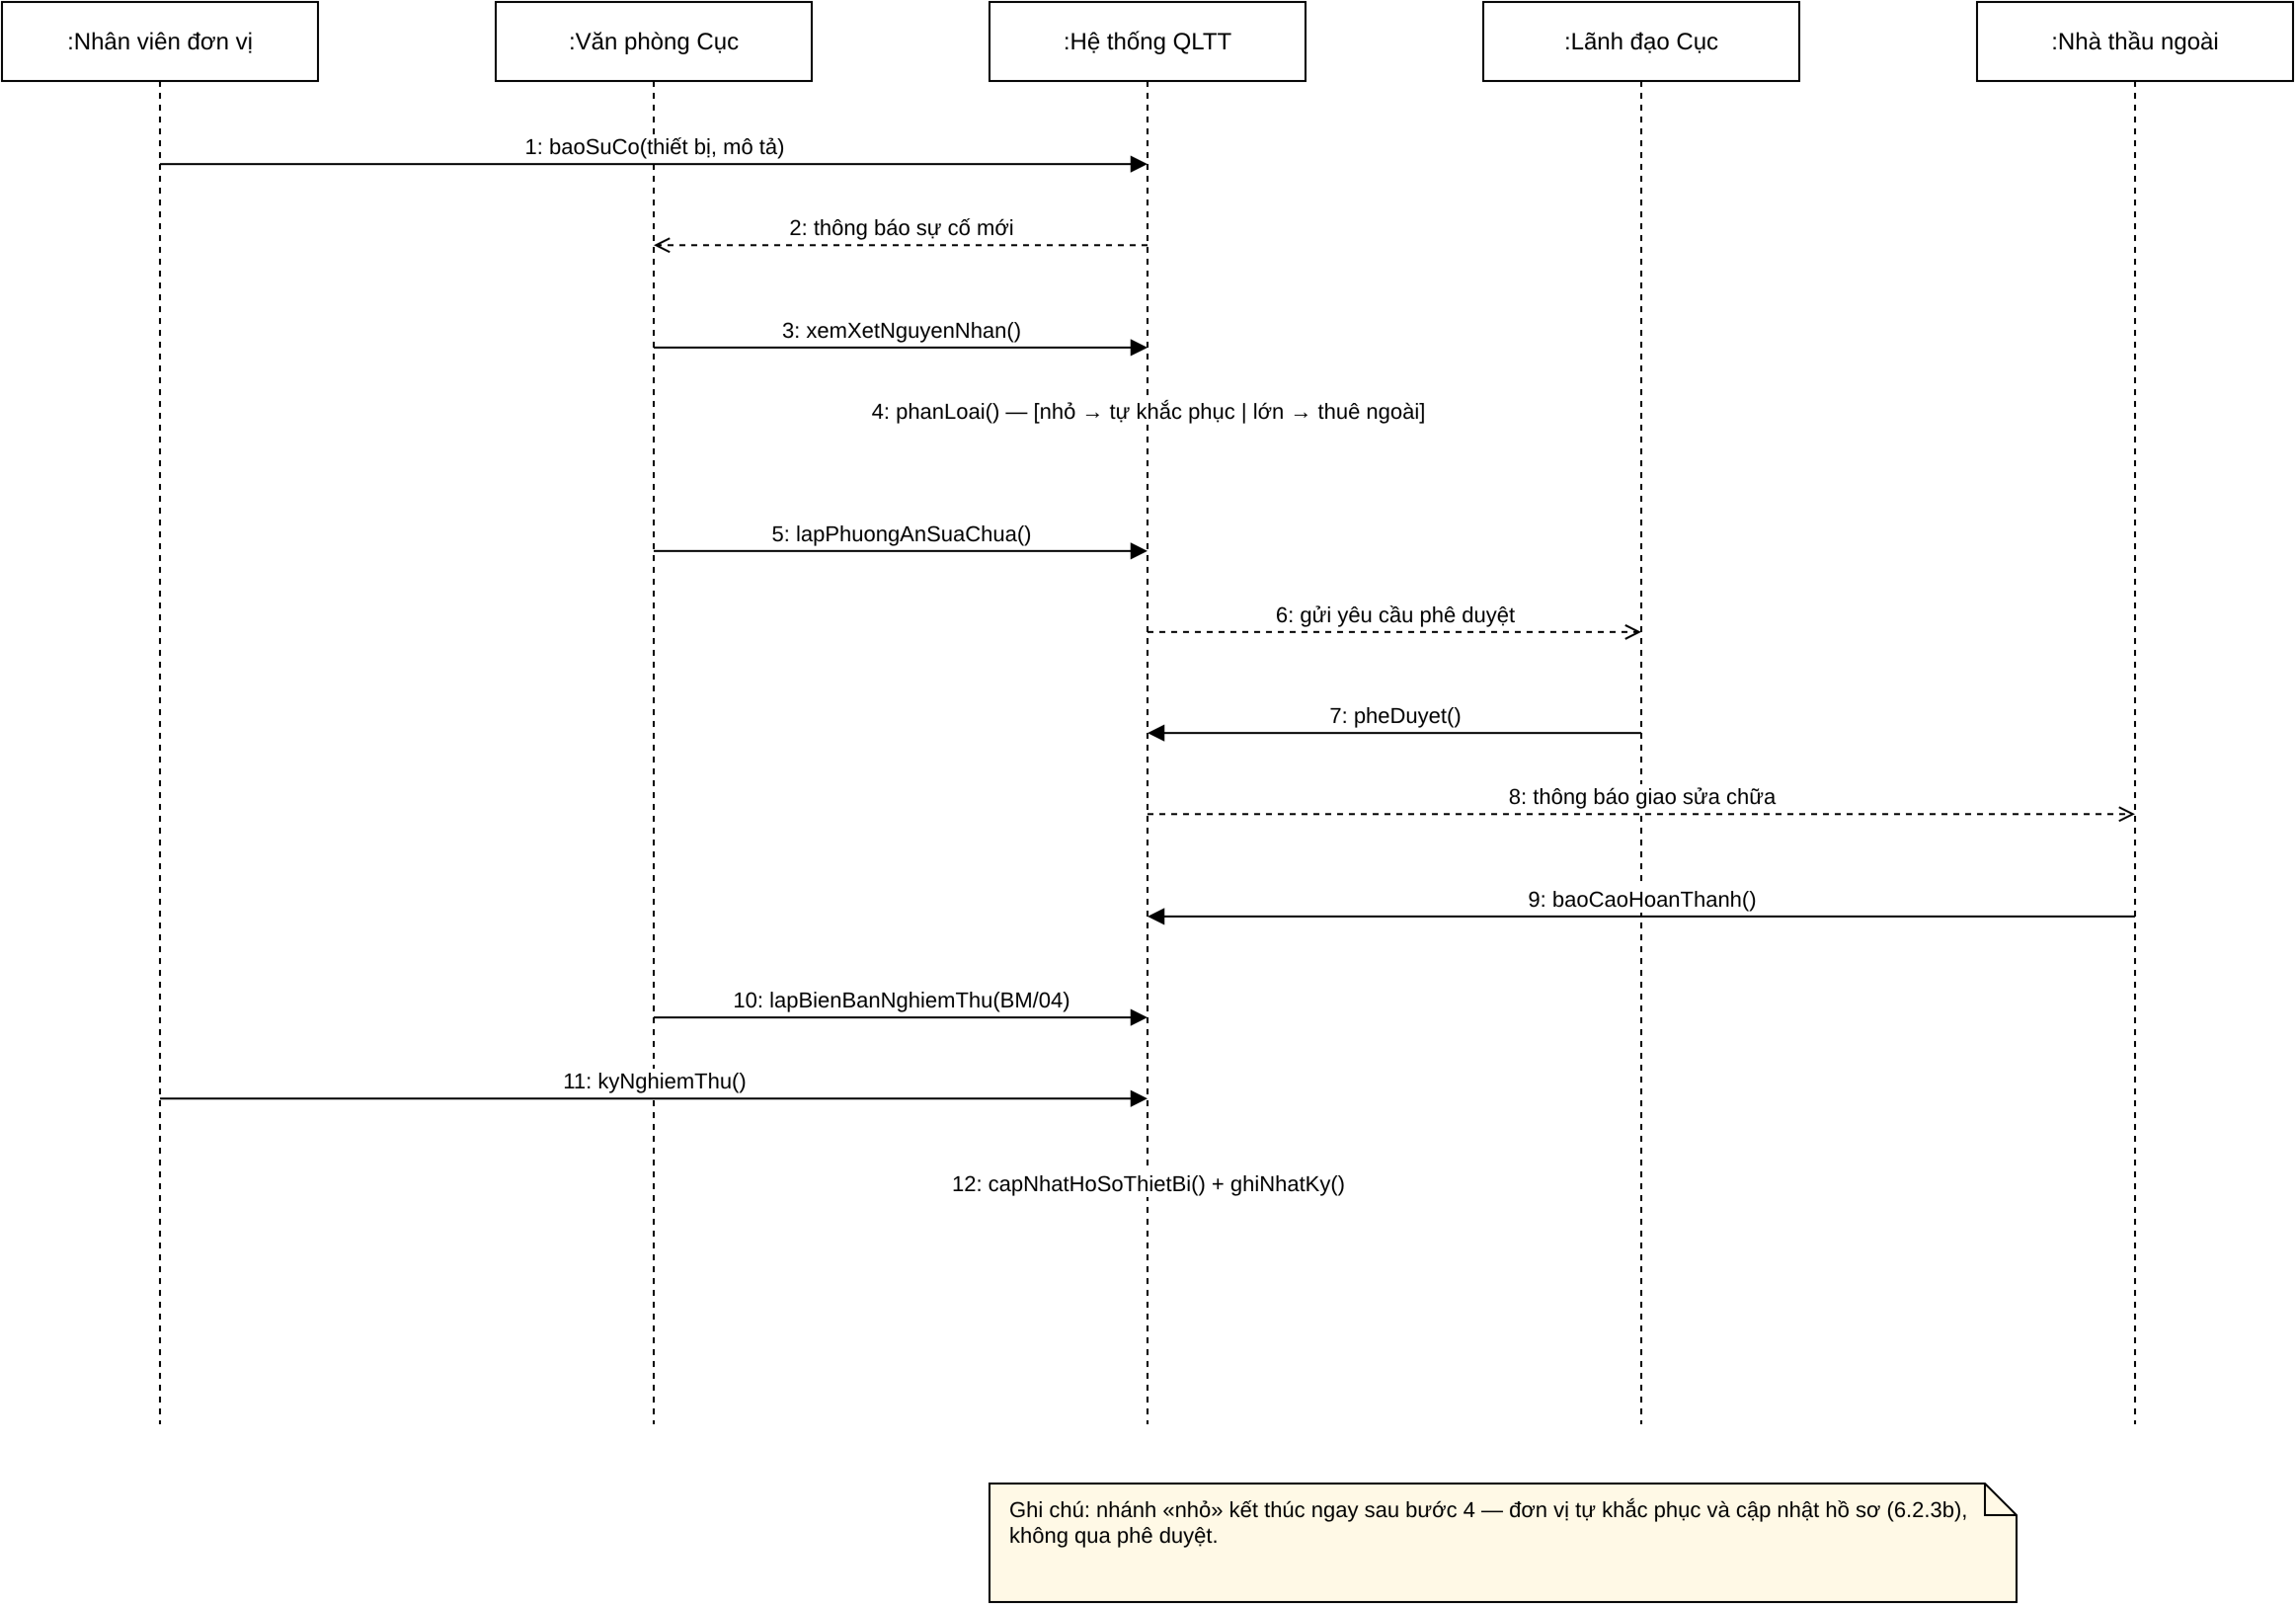
\includegraphics[width=0.94\textwidth]{figures/sequence-incident.png}}{\fbox{\parbox{0.9\textwidth}{\centering Sơ đồ trình tự xử lý sự cố (file \texttt{docs/diagrams/04-sequence.drawio}, trang 1)}}}
\caption{Sơ đồ trình tự — xử lý sự cố thuê ngoài}
\label{fig:seq-incident}
\end{figure}

Diễn giải Hình~\ref{fig:seq-incident}:
\begin{enumerate}
  \item Đơn vị gửi \texttt{baoSuCo(thiết bị, mô tả)}; hệ thống sinh mã sự cố, chuyển thiết bị sang ``Sự cố'' và thông báo cho Văn phòng Cục.
  \item Văn phòng Cục gọi \texttt{xemXetNguyenNhan()}; hệ thống \texttt{phanLoai()}: nếu nhỏ $\rightarrow$ kết thúc ngay (đơn vị tự khắc phục, không qua duyệt); nếu lớn $\rightarrow$ tiếp tục.
  \item Văn phòng Cục \texttt{lapPhuongAnSuaChua()}; hệ thống gửi yêu cầu phê duyệt tới Lãnh đạo Cục.
  \item Lãnh đạo Cục \texttt{pheDuyet()}; hệ thống thông báo giao sửa chữa cho nhà thầu, thiết bị chuyển ``Đang sửa chữa''.
  \item Nhà thầu \texttt{baoCaoHoanThanh()}; Văn phòng Cục \texttt{lapBienBanNghiemThu(BM/04)}; các bên \texttt{kyNghiemThu()}.
  \item Khi đủ chữ ký, hệ thống tự thực hiện \texttt{capNhatHoSoThietBi() + ghiNhatKy()} — đóng sự cố, trả thiết bị về ``Hoạt động''.
\end{enumerate}

\subsection{Lập và phê duyệt kế hoạch bảo dưỡng}

\begin{figure}[h]
\centering
\IfFileExists{figures/sequence-plan.png}{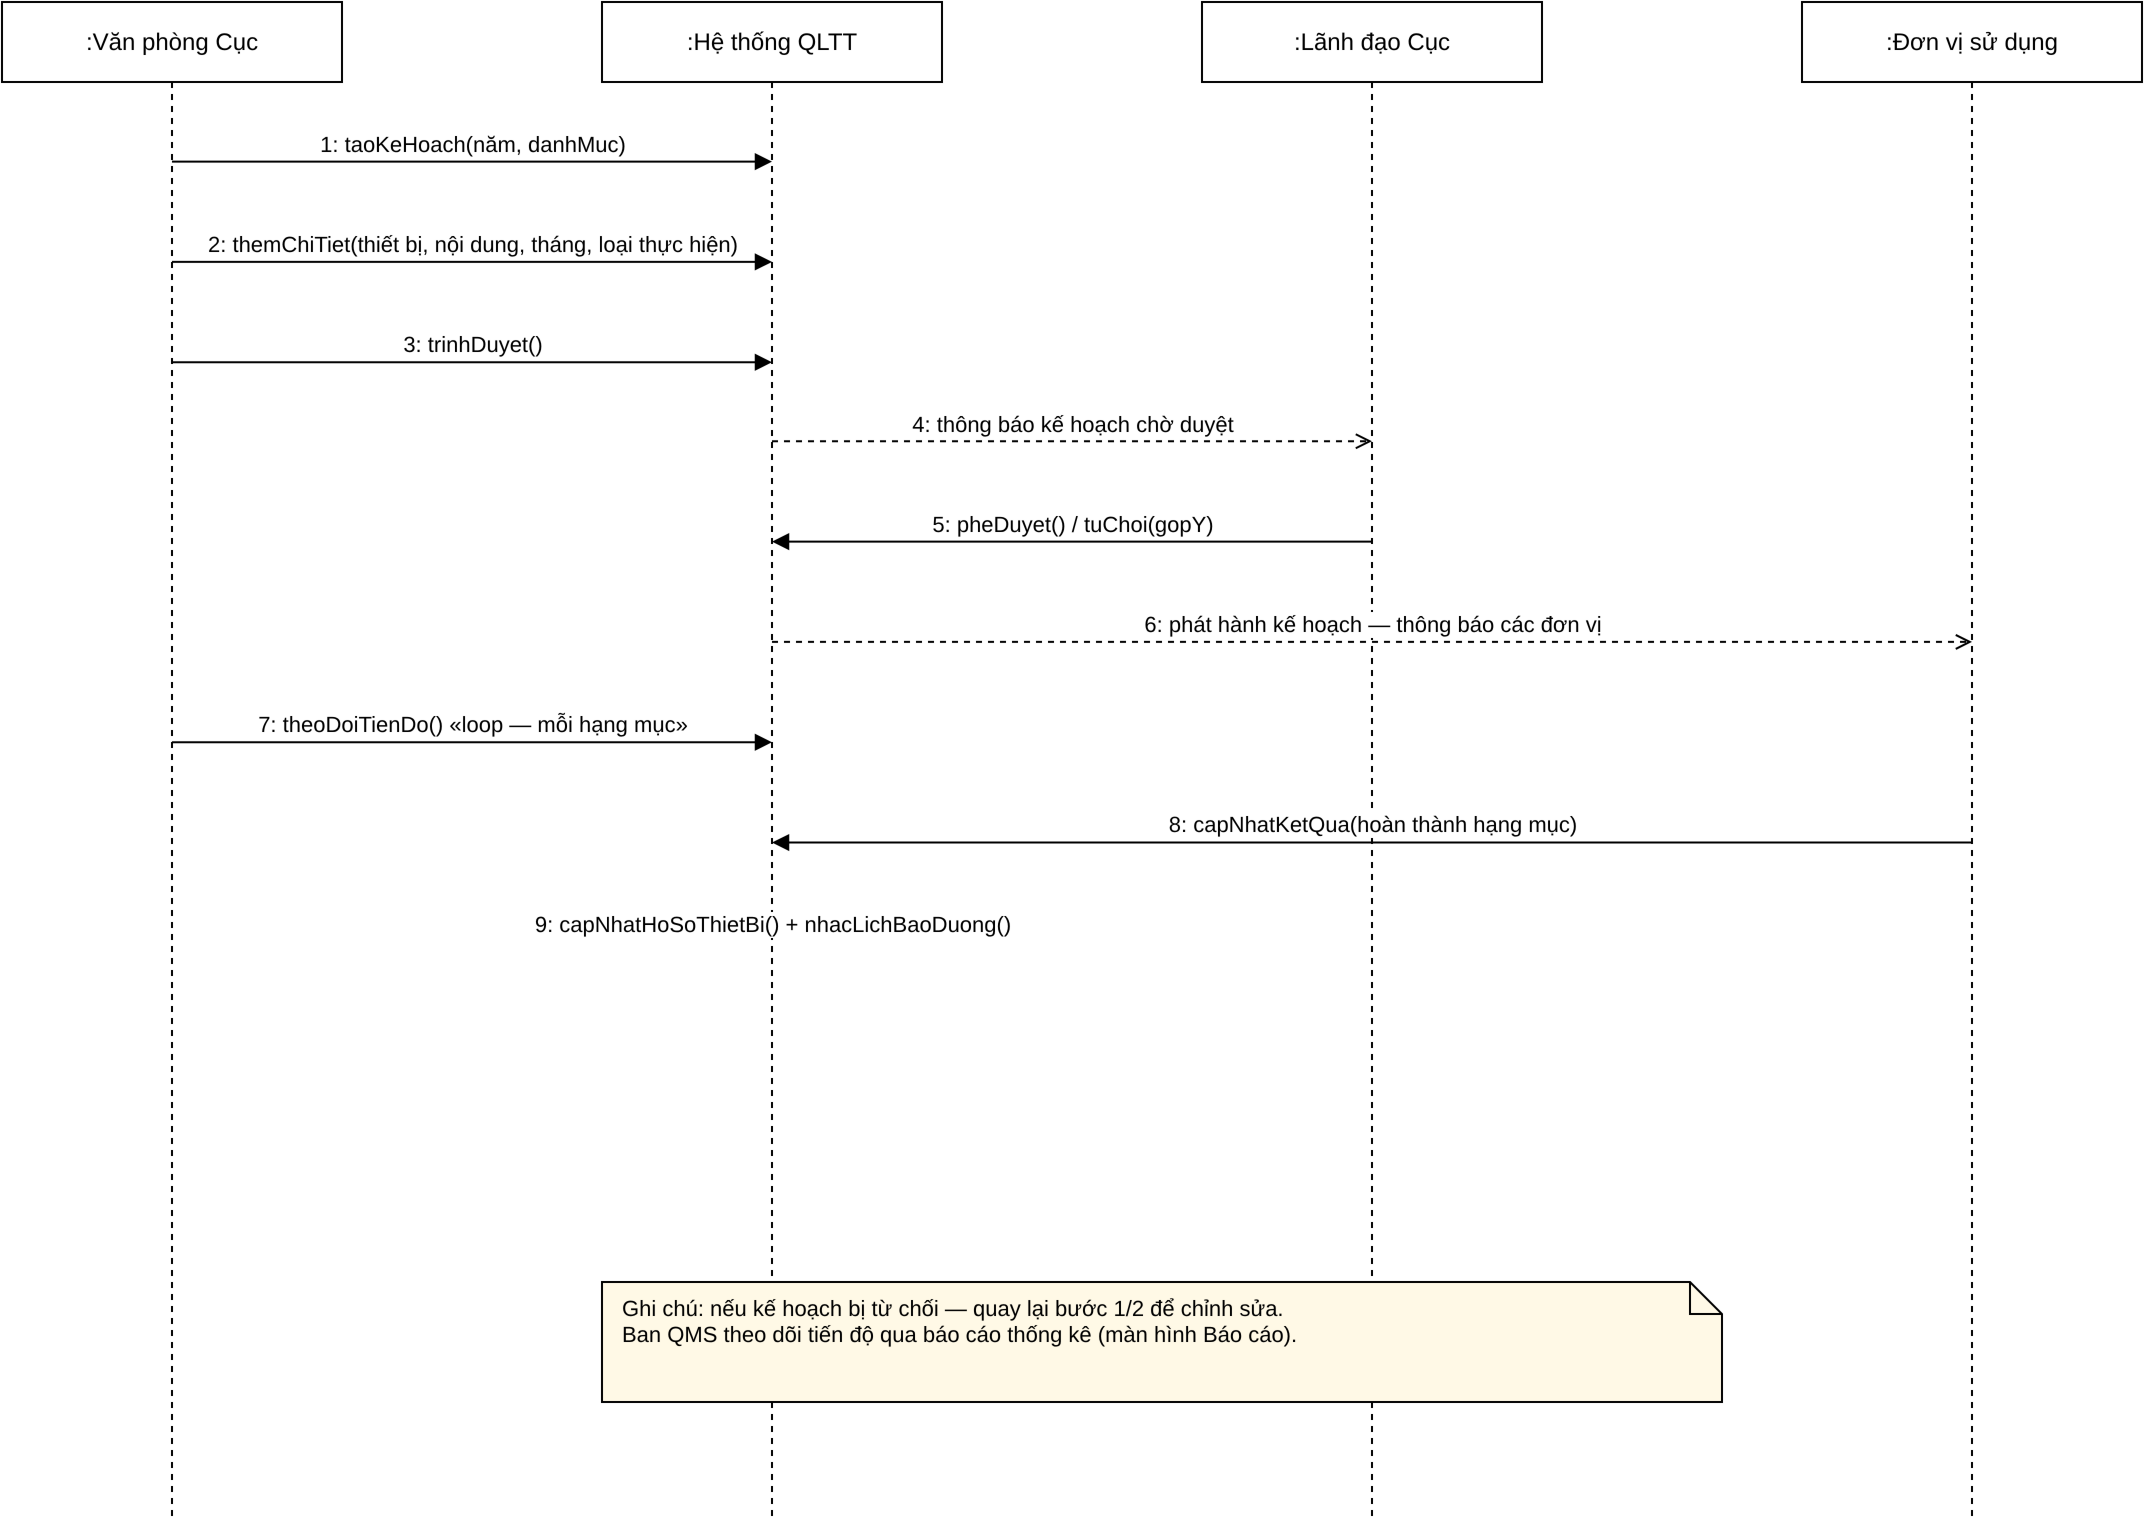
\includegraphics[width=0.9\textwidth]{figures/sequence-plan.png}}{\fbox{\parbox{0.9\textwidth}{\centering Sơ đồ trình tự kế hoạch bảo dưỡng (file \texttt{docs/diagrams/04-sequence.drawio}, trang 2)}}}
\caption{Sơ đồ trình tự — lập và phê duyệt kế hoạch hàng năm}
\label{fig:seq-plan}
\end{figure}

Diễn giải Hình~\ref{fig:seq-plan}: Văn phòng Cục \texttt{taoKeHoach(năm)} rồi \texttt{themChiTiet(...)} cho từng hạng mục (bước 1--2); \texttt{trinhDuyet()} (bước 3) đưa kế hoạch sang ``Chờ duyệt'' và thông báo Lãnh đạo Cục (bước 4). Lãnh đạo Cục \texttt{pheDuyet()/tuChoi(gopY)} (bước 5) — nếu bị từ chối thì quay lại bước 1--2 chỉnh sửa. Khi được duyệt, hệ thống phát hành kế hoạch tới các đơn vị (bước 6); vòng lặp theo dõi tiến độ (bước 7--8) kết thúc bằng \texttt{capNhatHoSoThietBi() + nhacLichBaoDuong()} (bước 9). Ban QMS theo dõi tiến độ qua màn hình báo cáo.

\section{Sơ đồ trạng thái}

\subsection{Vòng đời TrangThietBi}

\begin{figure}[h]
\centering
\IfFileExists{figures/state-equipment.png}{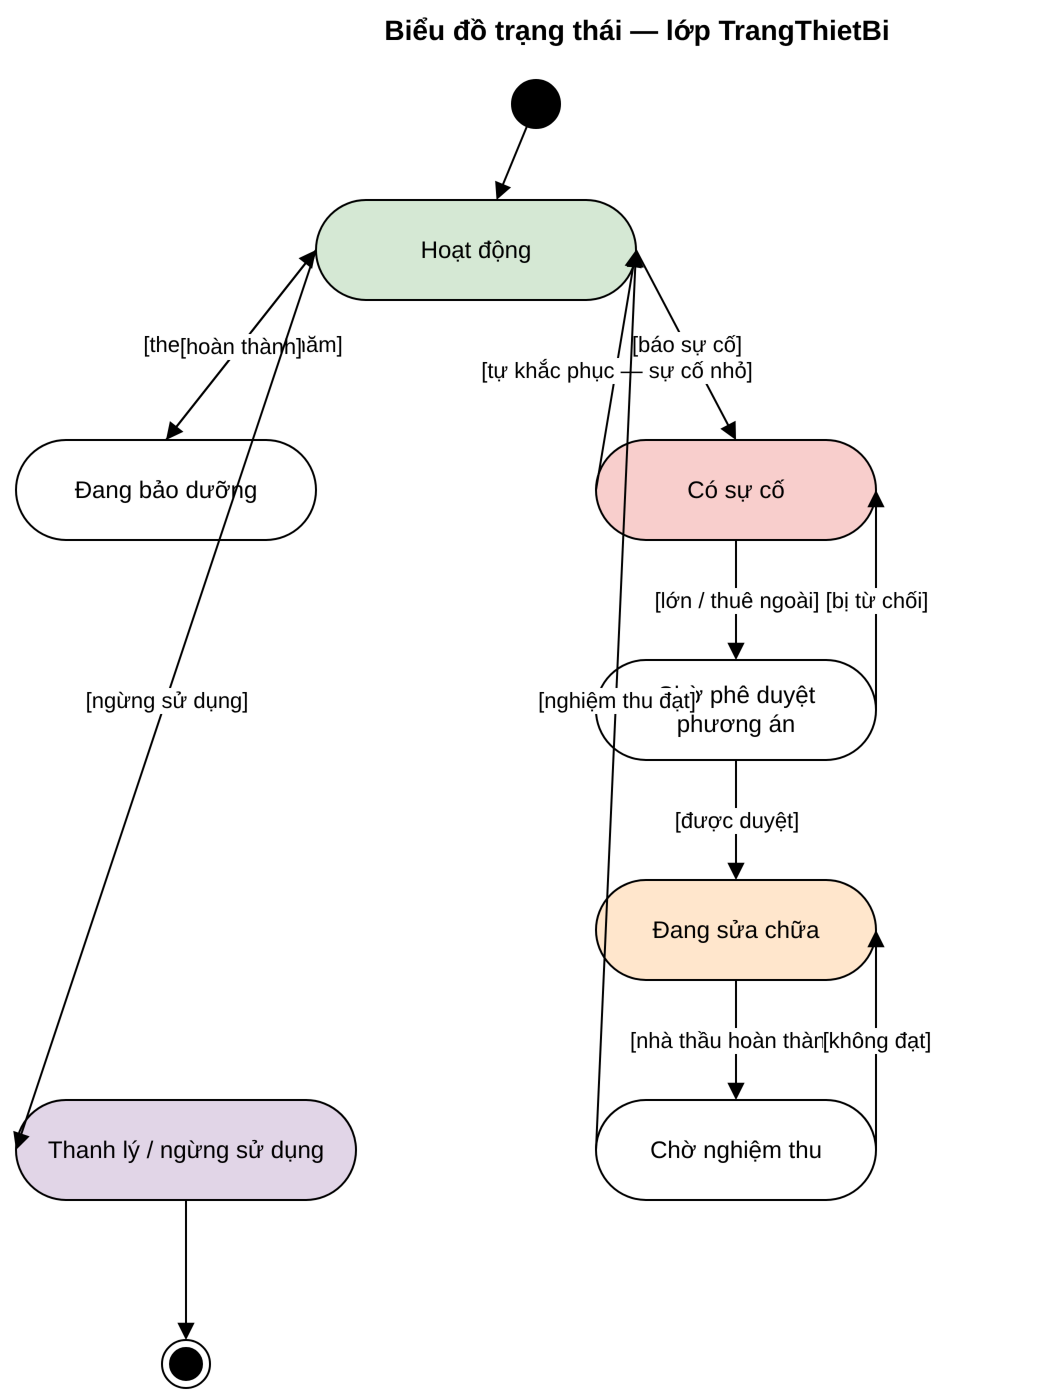
\includegraphics[width=0.72\textwidth]{figures/state-equipment.png}}{\fbox{\parbox{0.9\textwidth}{\centering Sơ đồ trạng thái TrangThietBi (file \texttt{docs/diagrams/05-state.drawio}, trang 1)}}}
\caption{Sơ đồ trạng thái của lớp TrangThietBi}
\label{fig:state-equip}
\end{figure}

\begin{table}[h]
\centering
\caption{Bảng chuyển tiếp trạng thái của TrangThietBi}
\label{tab:state-equip}
\begin{tabular}{P{2.6cm}P{3.4cm}P{9.2cm}}
\toprule
\textbf{Từ} & \textbf{Đến} & \textbf{Sự kiện / điều kiện} \\
\midrule
(bắt đầu) & Hoạt động & Thiết bị được đưa vào danh mục \\
Hoạt động & Đang bảo dưỡng & Theo kế hoạch năm đã duyệt (hạng mục bắt đầu) \\
Đang bảo dưỡng & Hoạt động & Hoàn thành hạng mục — tự ghi hồ sơ BM/02 \\
Hoạt động & Có sự cố & Đơn vị báo sự cố / nguy cơ \\
Có sự cố & Hoạt động & [sự cố nhỏ] Đơn vị tự khắc phục + cập nhật hồ sơ \\
Có sự cố & Chờ phê duyệt & [lớn / thuê ngoài] Chờ lập và duyệt phương án \\
Chờ phê duyệt & Đang sửa chữa & Lãnh đạo Cục phê duyệt phương án \\
Chờ phê duyệt & Có sự cố & Phương án bị từ chối \\
Đang sửa chữa & Chờ nghiệm thu & Nhà thầu/nội bộ báo hoàn thành \\
Chờ nghiệm thu & Hoạt động & Nghiệm thu đạt — đủ chữ ký biên bản BM/04 \\
Chờ nghiệm thu & Đang sửa chữa & Nghiệm thu không đạt \\
Hoạt động & Thanh lý / ngừng sử dụng & Quyết định ngừng sử dụng (hồ sơ BM/02 lưu đến khi máy không sử dụng) \\
Thanh lý & (kết thúc) & Tháo khỏi danh mục hoạt động \\
\bottomrule
\end{tabular}
\end{table}

\subsection{Vòng đời SuCo}

\begin{figure}[h]
\centering
\IfFileExists{figures/state-incident.png}{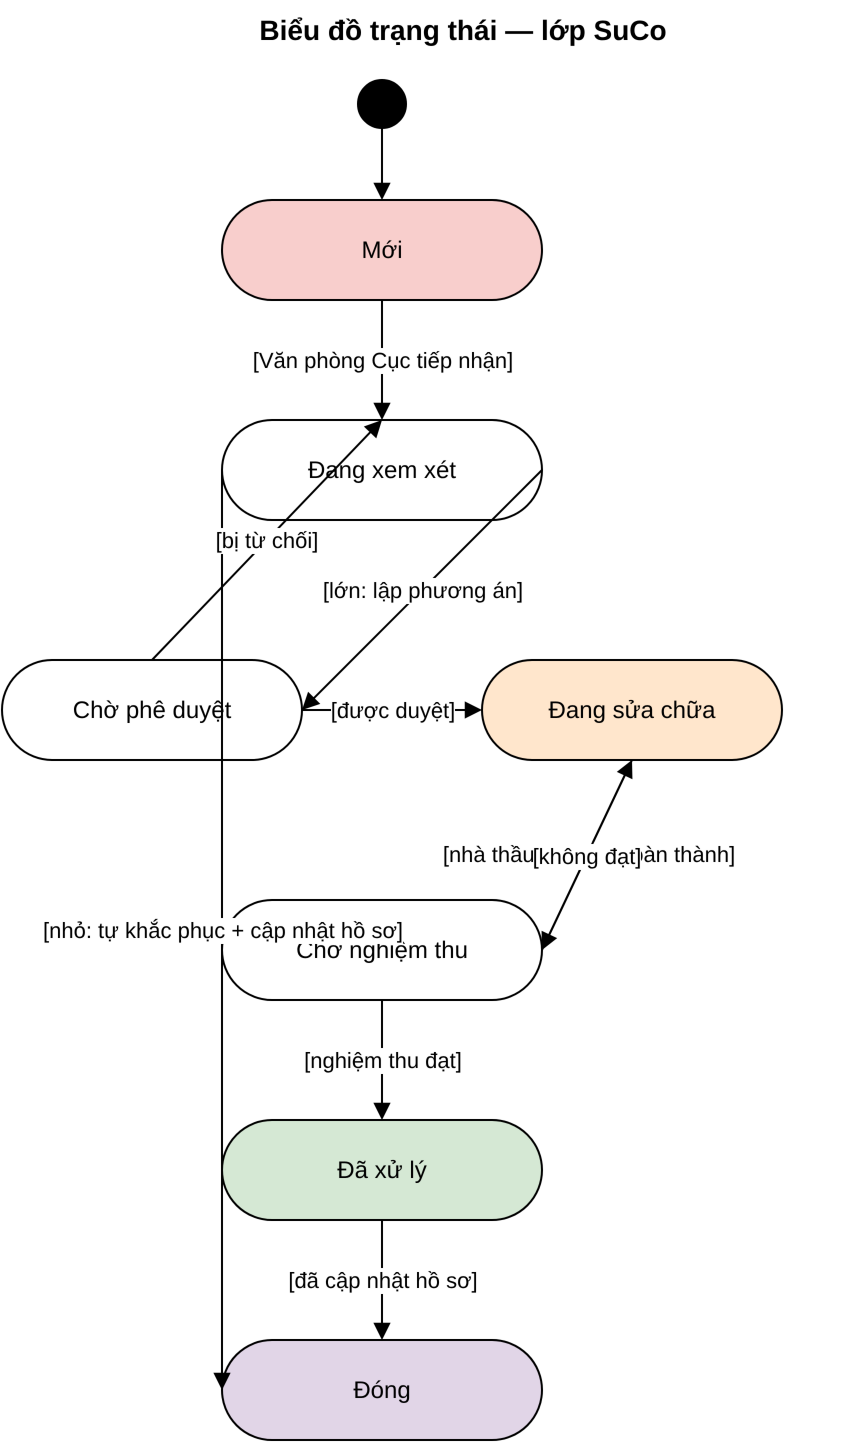
\includegraphics[width=0.72\textwidth]{figures/state-incident.png}}{\fbox{\parbox{0.9\textwidth}{\centering Sơ đồ trạng thái SuCo (file \texttt{docs/diagrams/05-state.drawio}, trang 2)}}}
\caption{Sơ đồ trạng thái của lớp SuCo}
\label{fig:state-incident}
\end{figure}

Điểm đáng chú ý của Hình~\ref{fig:state-incident}: từ ``Đang xem xét'' có hai đường rời đi phản ánh đúng quy trình — \textbf{[nhỏ: tự khắc phục + cập nhật hồ sơ]} đi thẳng tới ``Đóng'' (bỏ qua phê duyệt), còn \textbf{[lớn: lập phương án]} đi qua ``Chờ phê duyệt''. Trạng thái ``Chờ phê duyệt'' khi bị từ chối quay về ``Đang xem xét'' (lập lại phương án), không mất dữ liệu.

\section{Kết luận chương}

Ba loại sơ đồ hành vi (trình tự, trạng thái) được xây dựng cho hai luồng nghiệp vụ cốt lõi và hai lớp then chốt, bảo đảm: (i) nhất quán với sơ đồ use case (Chương 3) và sơ đồ lớp (Chương 4); (ii) đúng ngữ nghĩa quy trình gốc — đặc biệt nhánh sự cố nhỏ không qua phê duyệt; (iii) đủ cơ sở cho thiết kế state machine trong mã nguồn (Chương 6).

\chapter{Thiết kế hệ thống}

\section{Kiến trúc tổng thể}

Hệ thống được tổ chức theo \textbf{kiến trúc ba lớp} trên nền Docker Compose (5 container):

\begin{figure}[h]
\centering
\IfFileExists{figures/deployment.png}{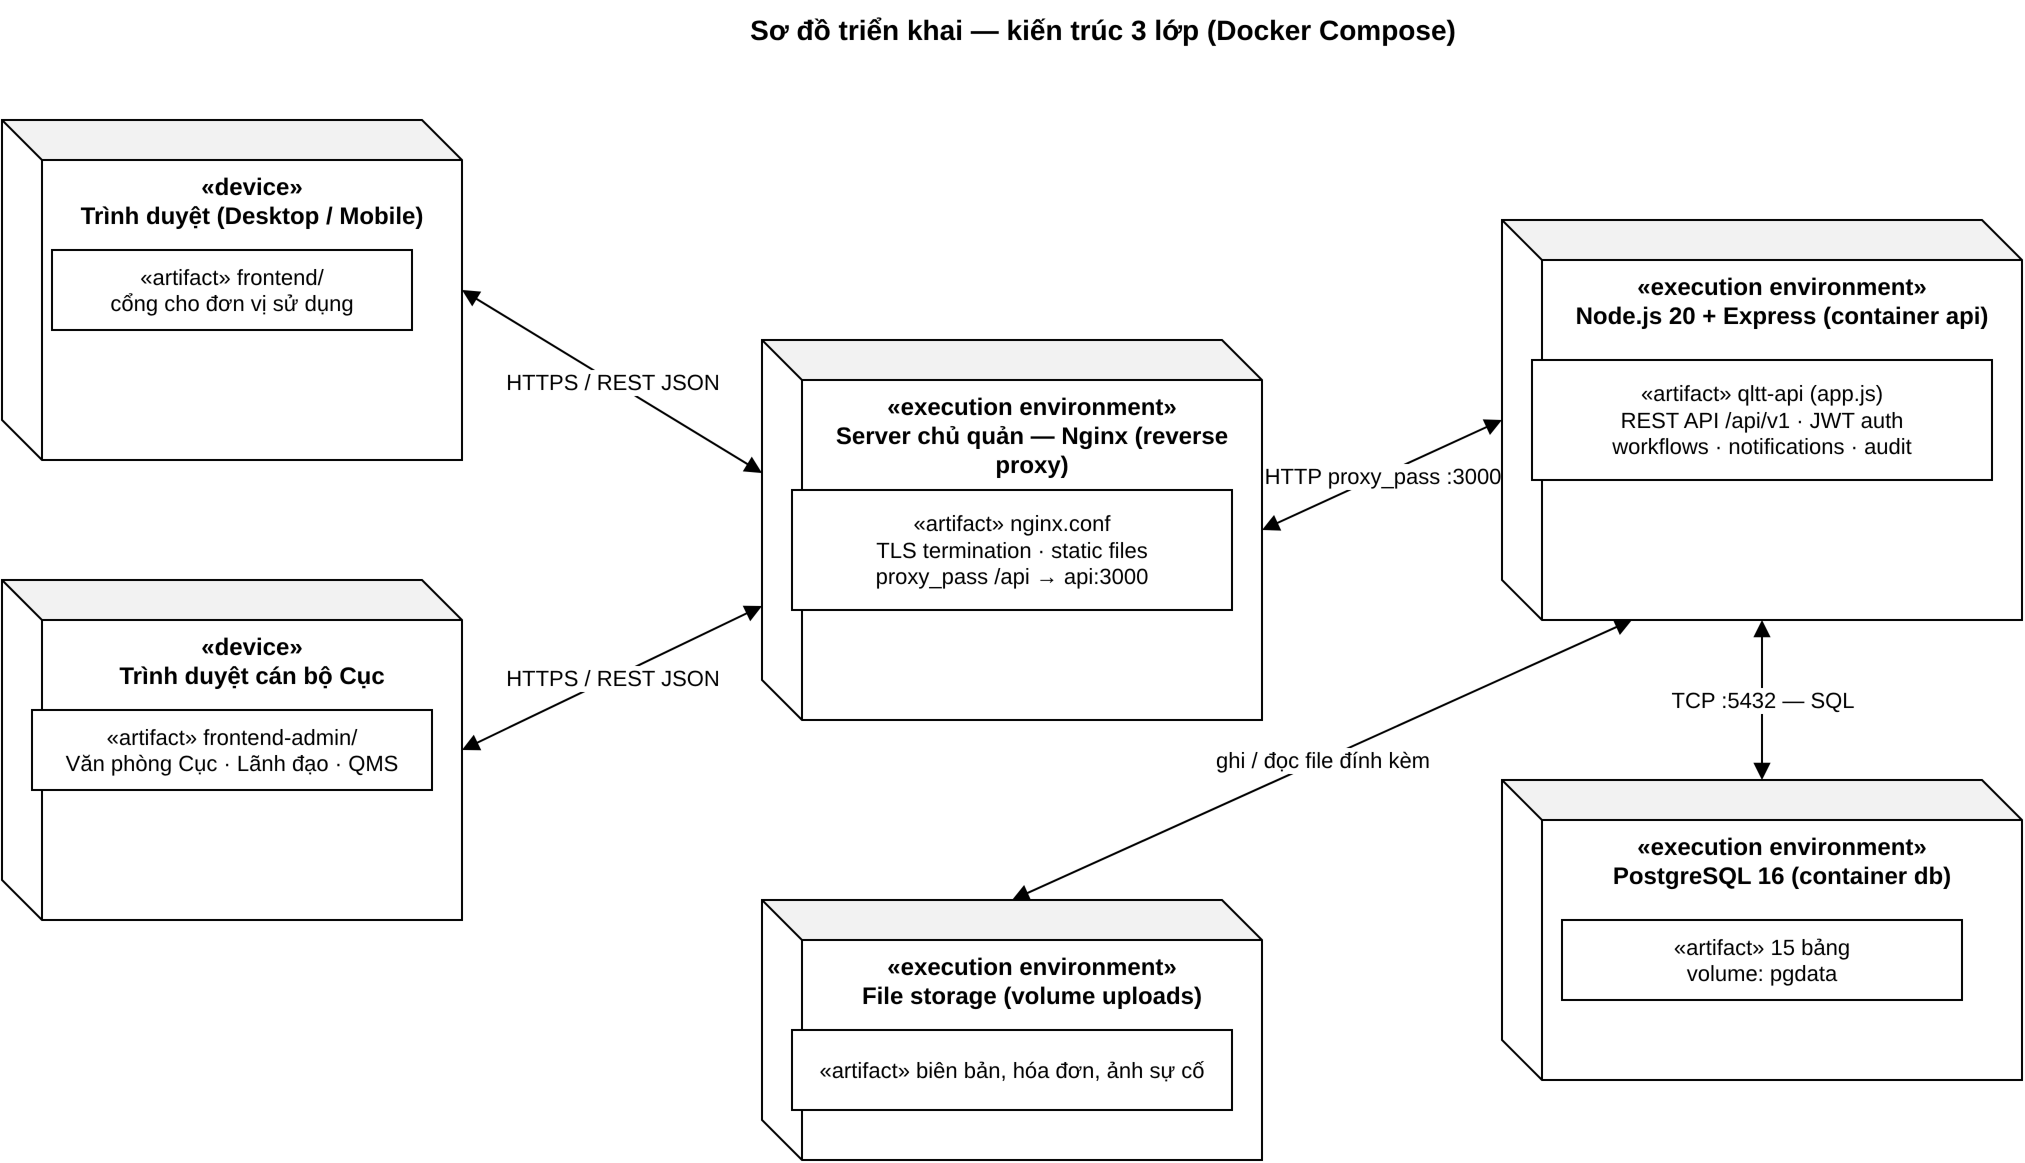
\includegraphics[width=0.96\textwidth]{figures/deployment.png}}{\fbox{\parbox{0.9\textwidth}{\centering Sơ đồ triển khai (file \texttt{docs/diagrams/06-erd-deployment.drawio}, trang 2)}}}
\caption{Sơ đồ triển khai — kiến trúc ba lớp}
\label{fig:deploy}
\end{figure}

\begin{table}[h]
\centering
\caption{Các thành phần triển khai}
\label{tab:components}
\begin{tabular}{P{3.4cm}P{5cm}P{6.6cm}}
\toprule
\textbf{Container} & \textbf{Công nghệ} & \textbf{Vai trò} \\
\midrule
frontend (nginx :8080) & Nginx + HTML/CSS/JS tĩnh & Cổng cho đơn vị sử dụng: tra cứu thiết bị, báo sự cố, theo dõi sự cố, xem kế hoạch \\
frontend-admin (nginx :8081) & Nginx + HTML/CSS/JS tĩnh & Workspace cho Văn phòng Cục / Lãnh đạo Cục / QMS: duyệt, xử lý, báo cáo \\
api (:3001$\rightarrow$3000) & Node.js 20 + Express & REST API \texttt{/api/v1}: nghiệp vụ, state machine phê duyệt, JWT, nhắc lịch (node-cron) \\
db & PostgreSQL 16 & 15 bảng dữ liệu; volume \texttt{pgdata} \\
uploads (volume) & Docker volume & File đính kèm: biên bản, hóa đơn, ảnh sự cố \\
\bottomrule
\end{tabular}
\end{table}

Hai cổng frontend đều proxy \texttt{/api} về container \texttt{api:3000} qua Nginx — trình duyệt chỉ gọi API bằng đường dẫn tương đối, giúp triển khai sau reverse proxy/TLS của server chủ quản mà không cần CORS riêng.

\section{Thiết kế cơ sở dữ liệu}

\begin{figure}[h]
\centering
\IfFileExists{figures/erd.png}{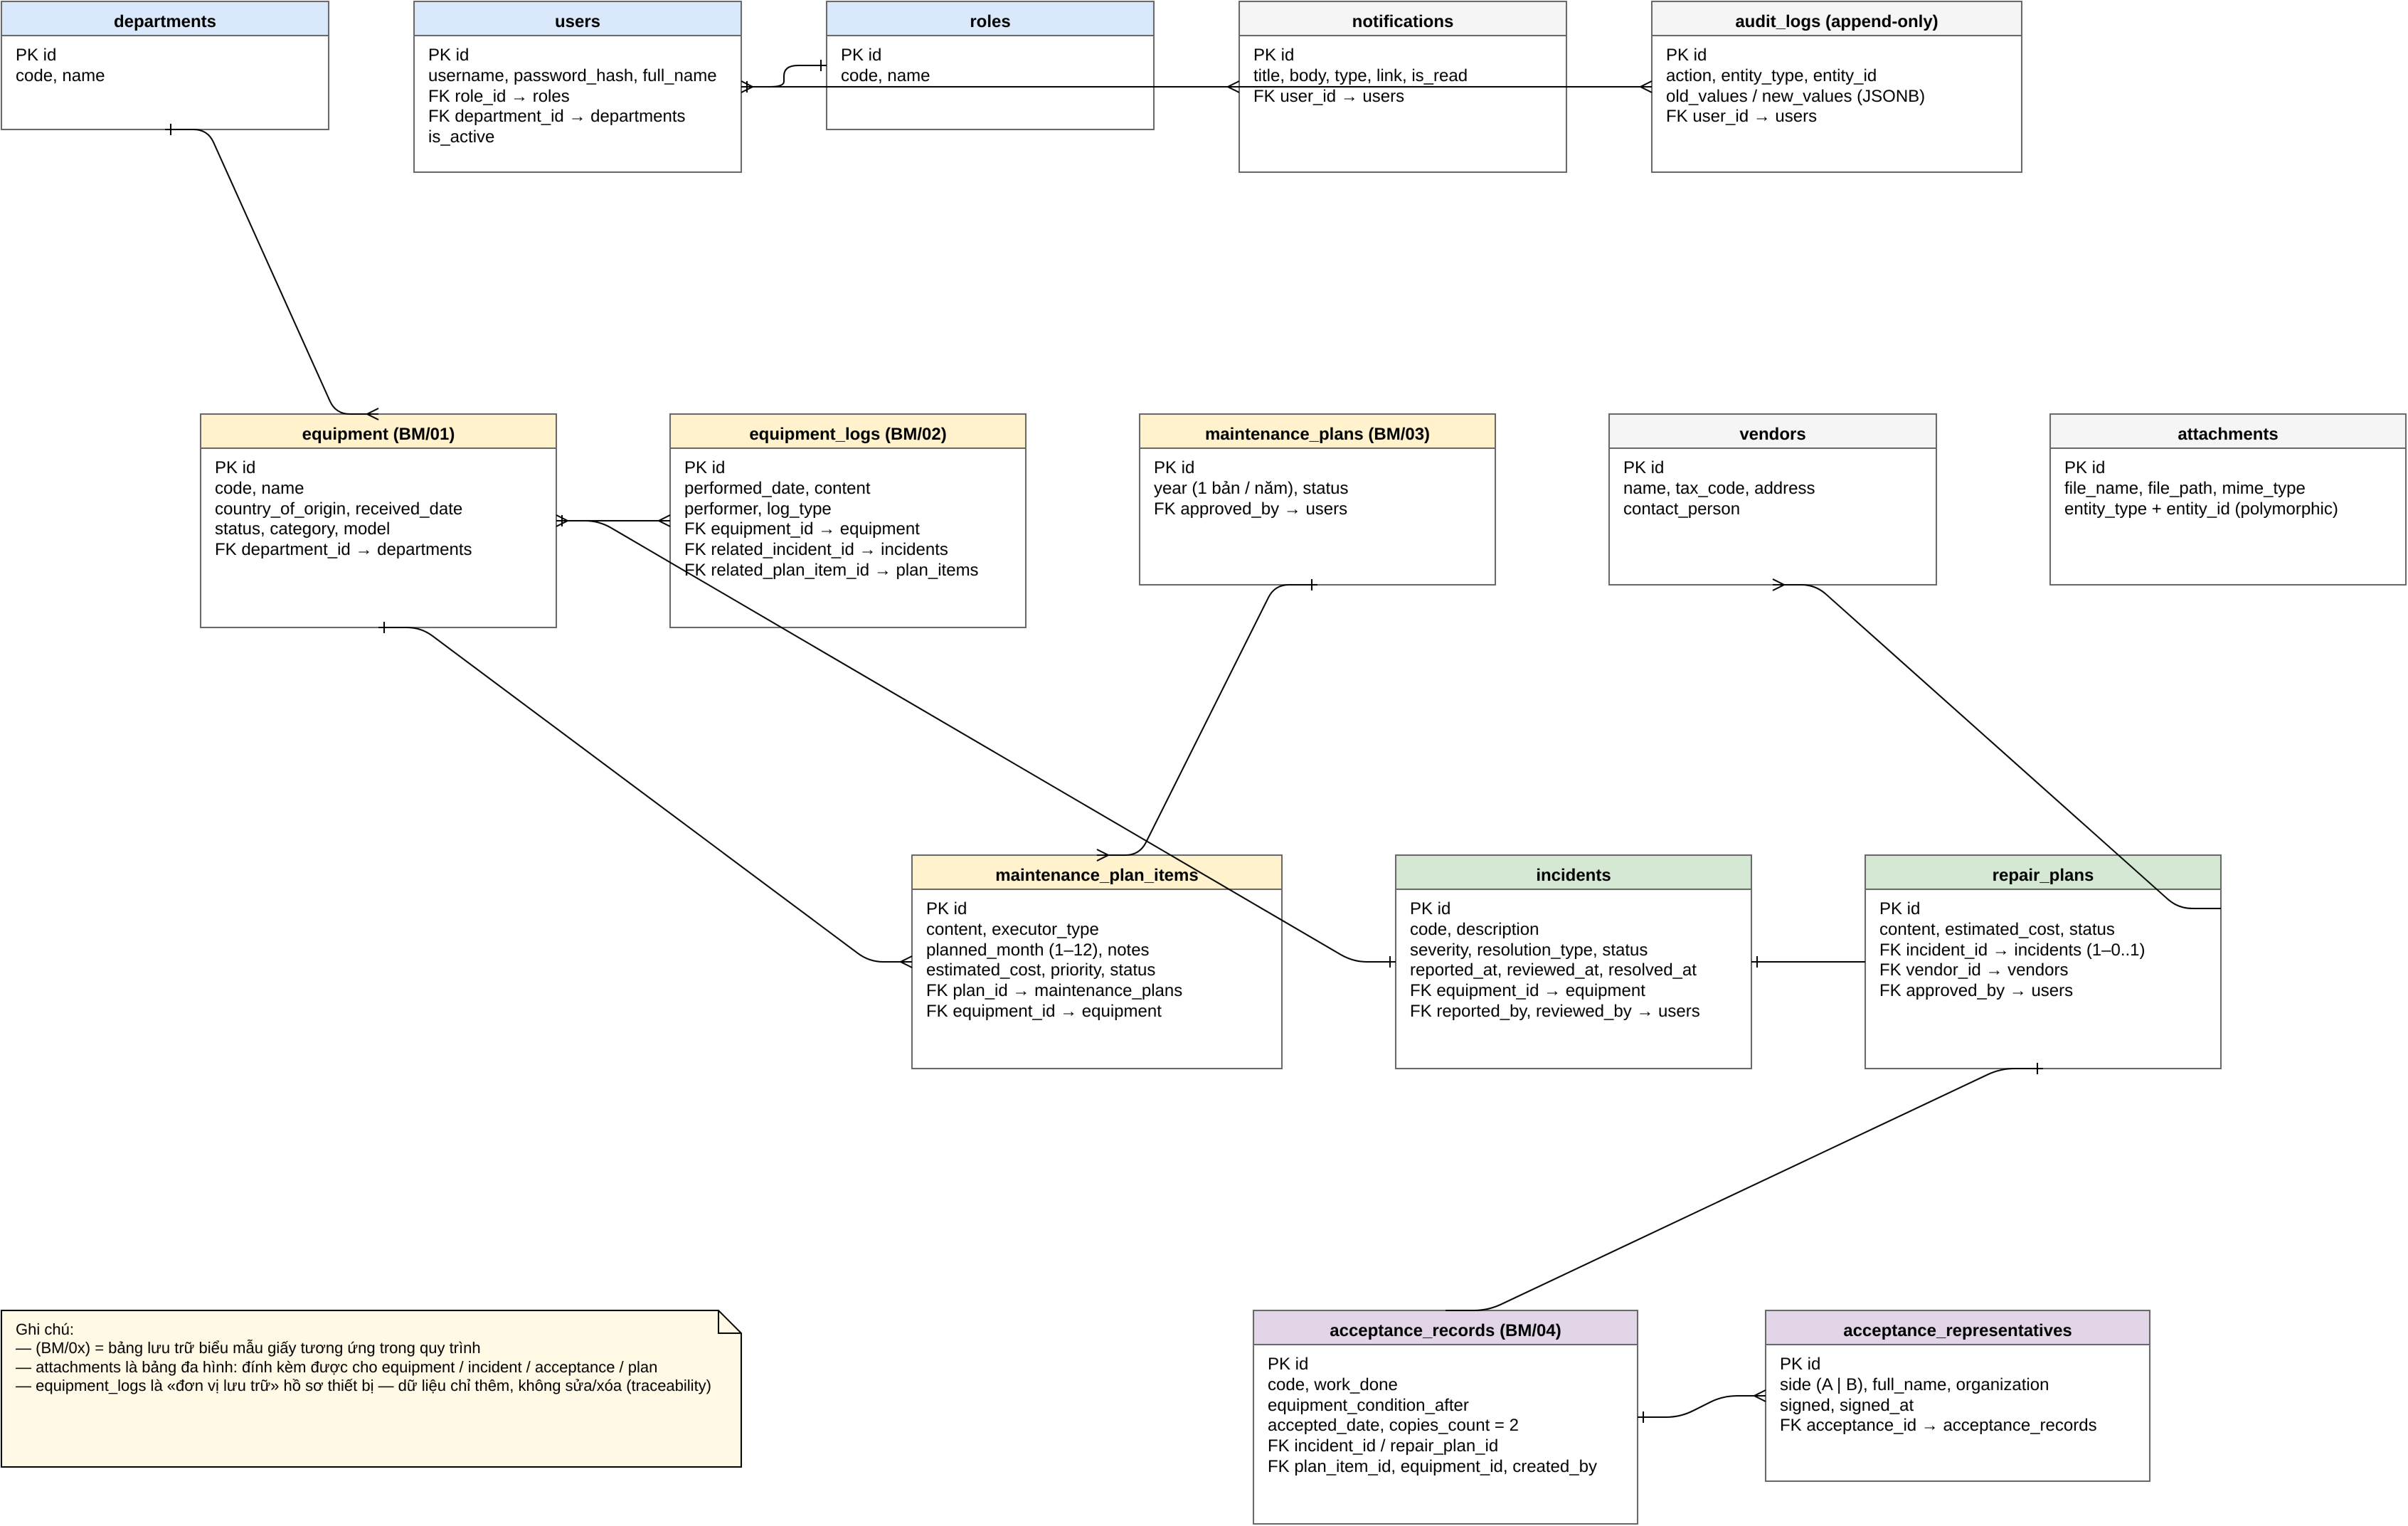
\includegraphics[width=\textwidth]{figures/erd.png}}{\fbox{\parbox{0.9\textwidth}{\centering ERD (file \texttt{docs/diagrams/06-erd-deployment.drawio}, trang 1)}}}
\caption{Sơ đồ thực thể — quan hệ (ERD) của cơ sở dữ liệu}
\label{fig:erd}
\end{figure}

Lược đồ gồm 15 bảng: \texttt{departments, roles, users, equipment, equipment\_logs, maintenance\_plans, maintenance\_plan\_items, incidents, repair\_plans, vendors, acceptance\_records, acceptance\_representatives, attachments, notifications, audit\_logs}. Các bảng cốt lõi:

\begin{longtable}{P{3.6cm}P{4.6cm}P{3cm}P{3.6cm}}
\caption{Lược đồ các bảng chính (nguồn gốc trường ghi trong ngoặc)}\label{tab:schema}\\
\toprule
\textbf{Bảng} & \textbf{Trường chính} & \textbf{Khóa ngoại} & \textbf{Nguồn gốc} \\
\midrule
\endfirsthead
\toprule
\textbf{Bảng} & \textbf{Trường chính} & \textbf{FK} & \textbf{Nguồn gốc} \\
\midrule
\endhead
equipment & code (Mã số), name (Tên), country\_of\_origin (Nước SX), received\_date (Ngày nhận), status [mở rộng] & department\_id & BM/01 \\
\addlinespace
equipment\_logs & performed\_date (Ngày thực hiện), content (Nội dung), performer (Người thực hiện), log\_type [mở rộng] & equipment\_id; related\_incident\_id; related\_plan\_item\_id & BM/02 \\
\addlinespace
maintenance\_plans & year (Năm, duy nhất), status, approved\_by, approval\_note & created\_by & BM/03 (header) \\
\addlinespace
maintenance\_plan\_items & content (Nội dung), executor\_type (nội bộ/bên ngoài), planned\_month (tháng), notes (Ghi chú); estimated\_cost, priority [mở rộng] & plan\_id; equipment\_id; department\_id & BM/03 (dòng) \\
\addlinespace
incidents & code [mở rộng], description, severity [mở rộng], resolution\_type, status, reported\_at & equipment\_id; reported\_by; reviewed\_by; department\_id & 6.2.3b \\
\addlinespace
repair\_plans & content, estimated\_cost [mở rộng], status phê duyệt & incident\_id (1--0..1); vendor\_id & 6.2.3b \\
\addlinespace
acceptance\_records & code, work\_done (đã thực hiện), equipment\_condition\_after (tình trạng sau), accepted\_date, copies\_count = 2 & incident\_id; repair\_plan\_id; plan\_item\_id; equipment\_id & BM/04 \\
\addlinespace
acceptance\_representatives & side (A/B), full\_name (Ông/bà), organization (Đơn vị), signed & acceptance\_id (hợp thành, CASCADE) & BM/04 \\
\addlinespace
audit\_logs & action, entity\_type, entity\_id, old\_values/new\_values (JSONB) & user\_id & ISO 9001 \\
\bottomrule
\end{longtable}

\textbf{Quy tắc thiết kế quan trọng:}
\begin{itemize}
  \item \texttt{equipment\_logs} và \texttt{audit\_logs} là hai bảng \emph{append-only}: ứng dụng không cung cấp UPDATE/DELETE — bảo đảm truy vết theo ISO 9001:2015.
  \item Trạng thái (status) được mã hóa bằng hằng số chuỗi có kiểm soát ở tầng API (state machine), không cho phép nhảy trạng thái tùy ý.
  \item \texttt{attachments} là bảng đa hình (entity\_type + entity\_id) — một cơ chế cho mọi loại đối tượng.
  \item Kế thừa TaiLieu được phẳng hóa (mục 4.4); hợp thành dựng bằng \texttt{ON DELETE CASCADE}.
\end{itemize}

\section{Thiết kế giao diện}

Hệ thống có \textbf{hai cổng} tách bạch theo đối tượng người dùng:

\begin{itemize}
  \item \textbf{Cổng đơn vị sử dụng} (theme tối, gold): trang chủ giới thiệu nghiệp vụ; tra cứu danh mục (đúng 6 cột BM/01); hồ sơ thiết bị dạng timeline (BM/02); form báo sự cố tối giản cho mobile; theo dõi sự cố của đơn vị với nút ``Tự khắc phục''; xem kế hoạch năm theo tab năm.
  \item \textbf{Cổng quản trị} (theme sáng, pastel): dashboard tổng quan với 4 thẻ số liệu thật và biểu đồ sự cố 12 tháng; bảng danh mục thiết bị + modal thêm/sửa + xuất Excel; xử lý sự cố (xem xét/phân loại, lập phương án); phương án sửa chữa (duyệt/từ chối/hoàn thành theo vai trò); kế hoạch năm (tạo nhiều hạng mục, trình duyệt, cập nhật tiến độ); nghiệm thu (lập biên bản với đại diện hai bên, ký); nhà thầu; người dùng \& phân quyền; báo cáo thống kê; nhật ký thao tác.
\end{itemize}

Nguyên tắc thiết kế: (i) bảng hiển thị \emph{giữ nguyên các cột của biểu mẫu giấy} để người dùng chuyển tiếp dễ; (ii) nút hành động chỉ hiện khi vai trò và trạng thái cho phép (UI phản ánh đúng state machine); (iii) responsive mobile-first cho luồng báo sự cố.

\section{Thiết kế bảo mật và kiểm soát tài liệu}

\begin{table}[h]
\centering
\caption{Ma trận phân quyền theo vai trò (tầng API)}
\label{tab:roles}
\begin{tabular}{P{4.4cm}P{10.6cm}}
\toprule
\textbf{Vai trò} & \textbf{Quyền} \\
\midrule
Đơn vị sử dụng & Xem thiết bị/hồ sơ của đơn vị mình; báo sự cố; tự khắc phục; cập nhật tiến độ hạng mục; ký biên bản (nếu là đại diện) \\
Văn phòng Cục & Toàn bộ CRUD danh mục/hồ sơ; xem xét sự cố; lập phương án/kế hoạch/biên bản; quản trị người dùng, nhà thầu; xuất Excel; xem nhật ký \\
Lãnh đạo Cục & Phê duyệt/từ chối kế hoạch và phương án; ký nghiệm thu; xem báo cáo \\
Ban QMS & Xem toàn bộ + báo cáo + nhật ký thao tác (không sửa nghiệp vụ) \\
Nhà thầu & Xem phương án liên quan; ký nghiệm thu (mở rộng) \\
\bottomrule
\end{tabular}
\end{table}

Cơ chế kỹ thuật: mật khẩu băm \texttt{bcrypt}; phiên \texttt{JWT} 8 giờ; middleware \texttt{authenticate} + \texttt{requireRole} chặn từng endpoint; middleware \texttt{attachAudit} ghi mọi thao tác quan trọng (CREATE/UPDATE/APPROVE/REJECT/SUBMIT/SIGN/LOGIN...) vào \texttt{audit\_logs} kèm dữ liệu cũ/mới dạng JSONB; file tải lên giới hạn 20MB, tải xuống qua route có xác thực.

\section{Thiết kế nhắc lịch và thông báo}

Job \texttt{node-cron} chạy \texttt{0 7 * * *}: truy vấn các hạng mục của kế hoạch \emph{đã duyệt} có tháng dự kiến trùng tháng hiện tại mà chưa hoàn thành $\rightarrow$ gửi thông báo cho Văn phòng Cục và các thành viên của đơn vị sử dụng liên quan. Thông báo trong hệ thống (\texttt{notifications}) đánh dấu đọc từng người dùng; chấm đỏ trên topbar phản ánh số chưa đọc.

\section{Thiết kế workflow (state machine trong mã nguồn)}

Thay vì BPM engine nặng, nhóm dùng state machine đơn giản: mỗi bản ghi có cột \texttt{status}; mỗi transition được cài đặt trong handler có kiểm tra trạng thái hiện tại (UPDATE ... WHERE status = ... RETURNING) — nếu không khớp trả 409. Điều này bảo đảm:
\begin{itemize}
  \item không thể duyệt một kế hoạch chưa trình, không thể ký biên bản đã ký;
  \item nhánh ``sự cố nhỏ'' được tối ưu: \texttt{review(TU\_KHAC\_PHUC)} $\rightarrow$ \texttt{self-resolve} $\rightarrow$ đóng, chỉ hai bước;
  \item mọi chuyển trạng thái đều phát sinh thông báo + audit log.
\end{itemize}

\chapter{Cài đặt thử nghiệm}

\section{Môi trường và cách triển khai}

Hệ thống được đóng gói và triển khai bằng Docker Compose với 5 container (Chương 6, Bảng~\ref{tab:components}). Lần đầu khởi động, container \texttt{api} tự chạy migration (\texttt{db/migrations/001\_init.sql}) và nạp dữ liệu mẫu bám theo quy trình (11 đơn vị, 5 vai trò, 6 thiết bị mẫu theo định nghĩa 5.1 của quy trình, kế hoạch năm 2026, sự cố, biên bản nghiệm thu).

\begin{verbatim}
# Khởi động toàn bộ hệ thống
docker compose up -d --build

# Cổng đơn vị sử dụng :  http://localhost:8080
# Cổng quản trị       :  http://localhost:8081
# API                 :  http://localhost:3001/api/v1/health
\end{verbatim}

\section{Kết quả thử nghiệm các luồng nghiệp vụ}

Hệ thống được thử nghiệm end-to-end qua API và giao diện. Kết quả:

\begin{table}[h]
\centering
\caption{Kết quả thử nghiệm các kịch bản chính}
\label{tab:test}
\begin{tabular}{P{0.8cm}P{8.6cm}P{3.2cm}P{2.2cm}}
\toprule
\textbf{STT} & \textbf{Kịch bản} & \textbf{Luồng kiểm chứng} & \textbf{Kết quả} \\
\midrule
1 & Đăng nhập 4 vai trò (đơn vị, Văn phòng Cục, Lãnh đạo Cục, QMS) & JWT trả về đúng vai trò; sai mật khẩu chặn 401 & Đạt \\
2 & Đơn vị báo sự cố nhỏ (máy in) & Mã SC-2026-xxx sinh tự động; thiết bị chuyển ``Sự cố''; VPC nhận thông báo & Đạt \\
3 & VPC xem xét, phân loại tự khắc phục; đơn vị tự khắc phục & Không qua phê duyệt; hồ sơ BM/02 tự thêm bản ghi; sự cố đóng; thiết bị về ``Hoạt động'' & Đạt \\
4 & Đơn vị báo sự cố lớn $\rightarrow$ VPC lập phương án thuê ngoài $\rightarrow$ Lãnh đạo Cục phê duyệt & Thiết bị chuyển ``Đang sửa chữa''; từ chối không ghi lý do bị chặn & Đạt \\
5 & Báo hoàn thành $\rightarrow$ lập biên bản BM/04 (2 bên đại diện) $\rightarrow$ ký đủ & Sự cố đóng; hồ sơ thiết bị thêm bản ghi ``Sửa chữa''; thiết bị về ``Hoạt động'' & Đạt \\
6 & Lập kế hoạch năm 2026 (4 hạng mục) $\rightarrow$ trình $\rightarrow$ phê duyệt & Trạng thái Nháp $\rightarrow$ Chờ duyệt $\rightarrow$ Đã duyệt; thông báo gửi đúng vai trò & Đạt \\
7 & Hoàn thành hạng mục bảo dưỡng theo kế hoạch & Tự ghi hồ sơ BM/02; thiết bị trả về ``Hoạt động'' & Đạt \\
8 & Xuất danh mục Excel (BM/01) & File .xlsx đúng 6 cột biểu mẫu & Đạt \\
9 & Phân quyền: đơn vị cố sửa thiết bị (403), QMS cố duyệt (403) & Middleware \texttt{requireRole} chặn đúng & Đạt \\
10 & Nhật ký thao tác & Mọi thao tác tạo/duyệt/ký/đăng nhập được ghi audit trail append-only & Đạt \\
\bottomrule
\end{tabular}
\end{table}

\section{Ảnh chụp màn hình hệ thống}

\begin{figure}[h]
\centering
\IfFileExists{figures/screen-admin-dashboard.png}{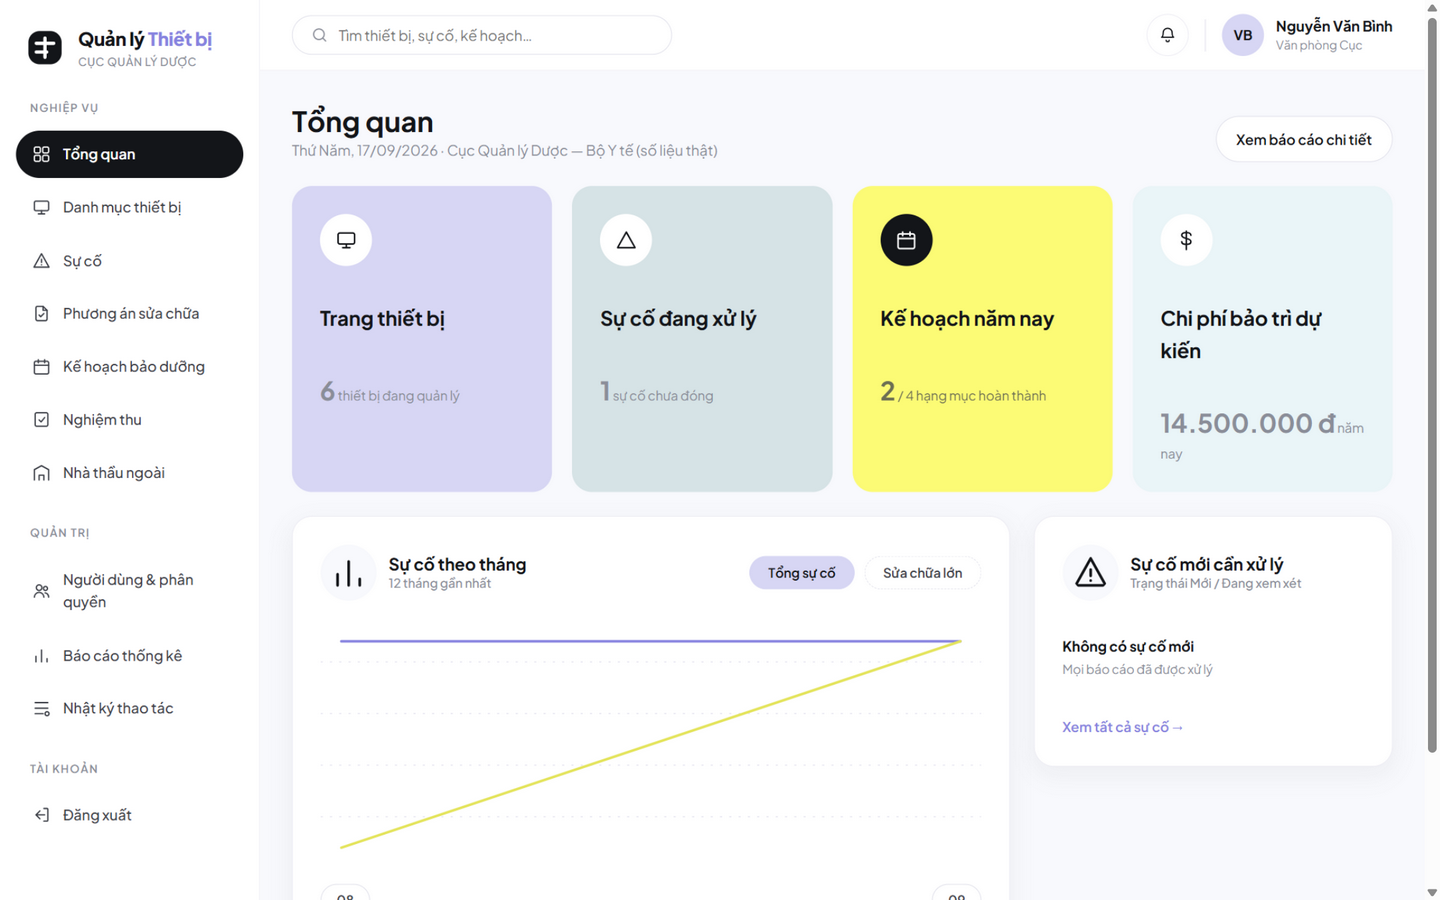
\includegraphics[width=\textwidth]{figures/screen-admin-dashboard.png}}{\fbox{\parbox{0.9\textwidth}{\centering Dashboard quản trị (xem demo trực tiếp tại cổng quản trị)}}}
\caption{Cổng quản trị — dashboard tổng quan với số liệu thật}
\label{fig:scr-dash}
\end{figure}

\begin{figure}[h]
\centering
\IfFileExists{figures/screen-user-home.png}{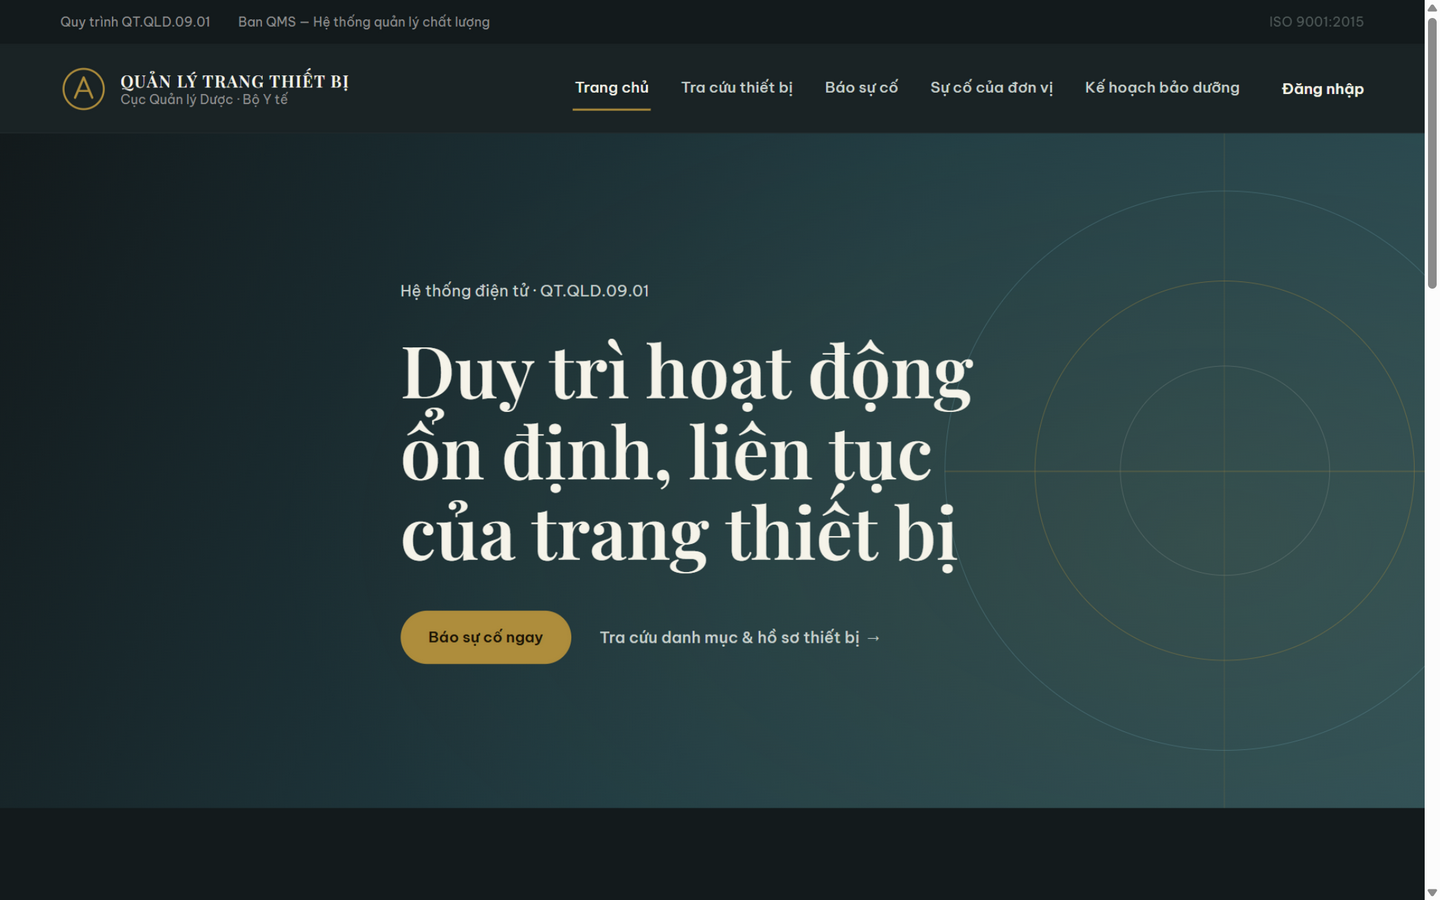
\includegraphics[width=\textwidth]{figures/screen-user-home.png}}{\fbox{\parbox{0.9\textwidth}{\centering Trang chủ cổng đơn vị sử dụng}}}
\caption{Cổng đơn vị sử dụng — trang chủ và tra cứu nhanh}
\label{fig:scr-home}
\end{figure}

\begin{figure}[h]
\centering
\IfFileExists{figures/screen-profile.png}{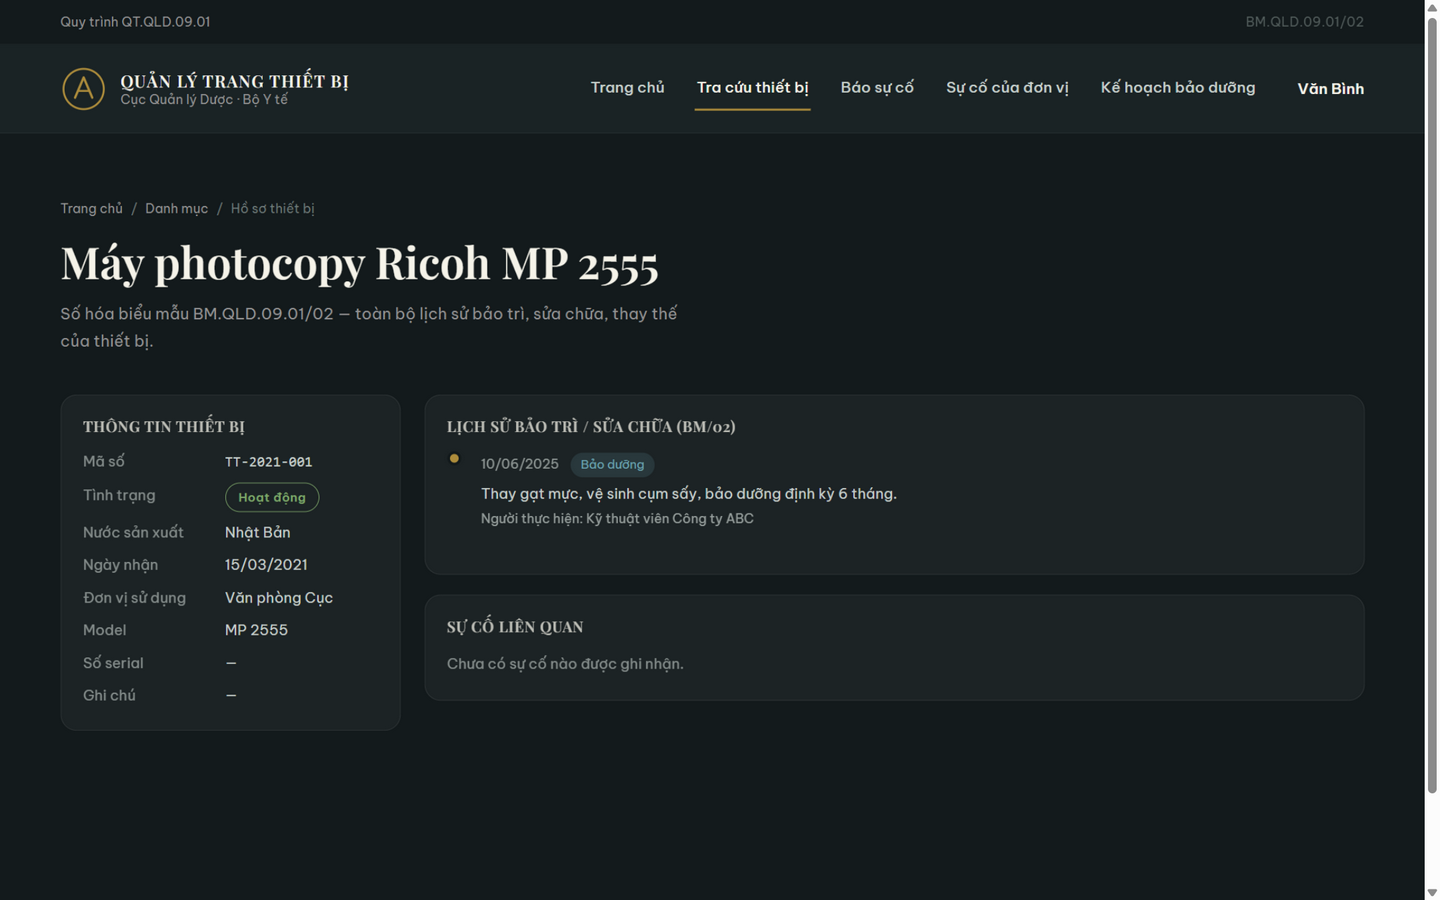
\includegraphics[width=\textwidth]{figures/screen-profile.png}}{\fbox{\parbox{0.9\textwidth}{\centering Hồ sơ thiết bị dạng timeline (BM/02)}}}
\caption{Hồ sơ trang thiết bị — timeline lịch sử bảo trì, sửa chữa}
\label{fig:scr-profile}
\end{figure}

\begin{figure}[h]
\centering
\IfFileExists{figures/screen-acceptance.png}{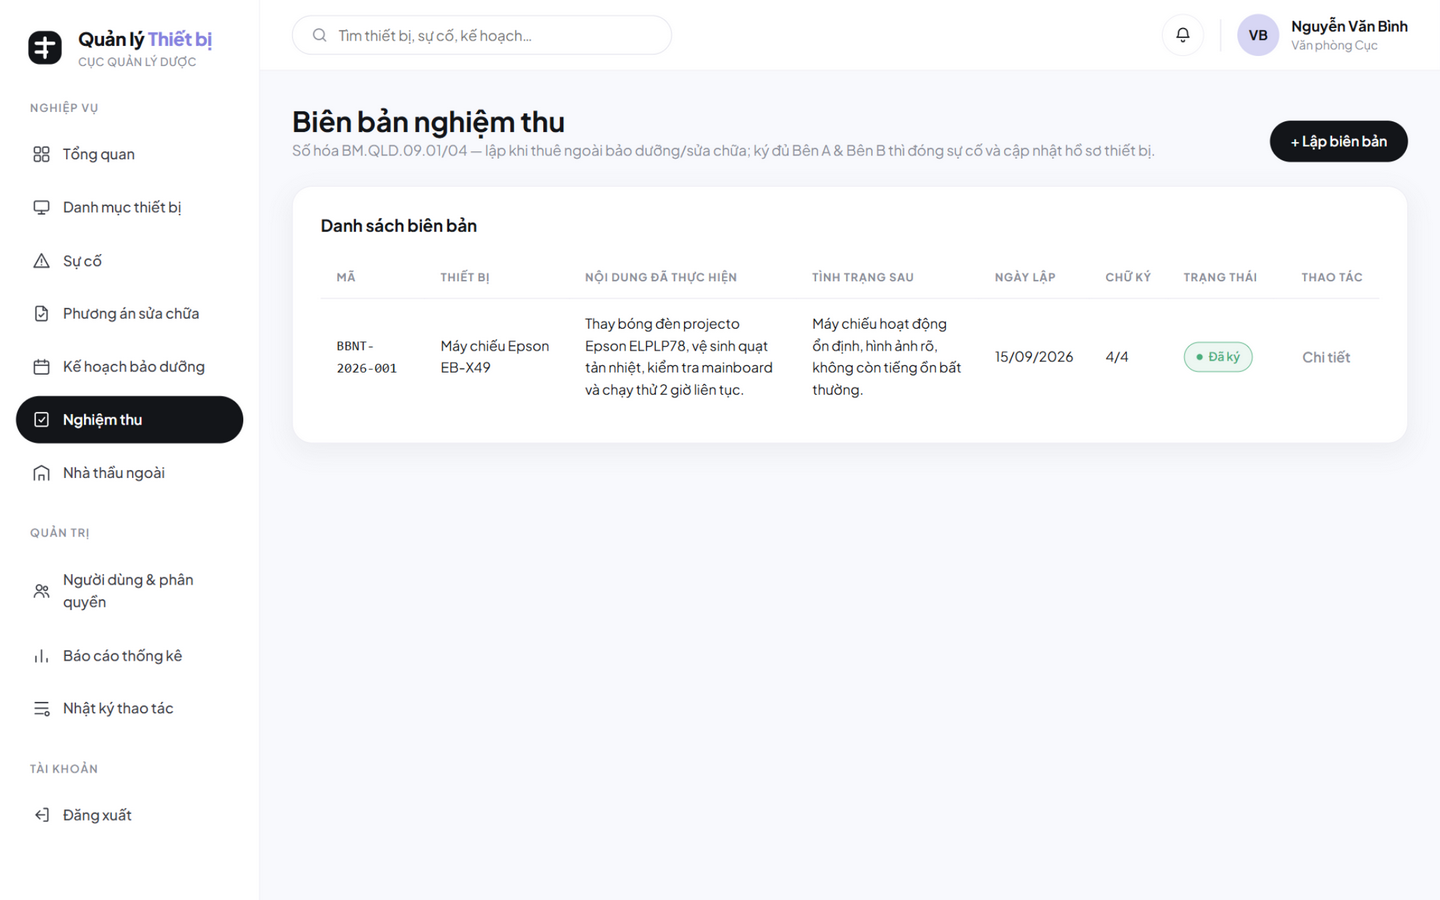
\includegraphics[width=\textwidth]{figures/screen-acceptance.png}}{\fbox{\parbox{0.9\textwidth}{\centering Danh sách biên bản nghiệm thu (BM/04)}}}
\caption{Nghiệm thu điện tử — theo dõi tiến độ ký của hai bên}
\label{fig:scr-acc}
\end{figure}

\section{Giới hạn của nguyên mẫu}

\begin{itemize}
  \item Chữ ký điện tử hiện là mô phỏng (ghi nhận tên + thời điểm), chưa tích hợp chữ ký số theo Nghị định 130/2020/NĐ-CP.
  \item Chưa chạy song song với biểu mẫu giấy trong môi trường thật; kịch bản chuyển đổi cần Ban QMS phê duyệt.
  \item Chưa đo lường chính thức hiệu năng và tải; chưa có bộ kiểm thử tự động hóa đầy đủ (hiện thử nghiệm thủ công theo Bảng~\ref{tab:test}).
\end{itemize}

\chapter{Kết luận và hướng phát triển}

\section{Kết quả đạt được}

So với mục tiêu đặt ra ở Chương 1, hệ thống đã đáp ứng:

\begin{table}[h]
\centering
\caption{Đối chiếu mục tiêu --- kết quả}
\label{tab:goals}
\begin{tabular}{P{0.8cm}P{7.4cm}P{6.6cm}}
\toprule
\textbf{TT} & \textbf{Mục tiêu} & \textbf{Kết quả} \\
\midrule
1 & Số hóa 4 biểu mẫu BM/01--/04 & 15 bảng CSDL bám đúng trường dữ liệu nguyên văn; giao diện tái hiện cột biểu mẫu; xuất Excel BM/01 \\
2 & Tự động hóa luồng phê duyệt & State machine Kế hoạch/Phương án: trình $\rightarrow$ duyệt/từ chối kèm lý do; thông báo tự động theo vai trò \\
3 & Cảnh báo, nhắc lịch & Job 07:00 hằng ngày nhắc hạng mục tháng hiện tại chưa hoàn thành \\
4 & Truy vết lịch sử thiết bị & Timeline hồ sơ BM/02 tự ghi từ mọi luồng; audit trail append-only \\
5 & Báo cáo cho QMS, Lãnh đạo & 5 báo cáo: tổng quan, thiết bị theo đơn vị, tần suất sự cố, tiến độ kế hoạch, nhật ký \\
\bottomrule
\end{tabular}
\end{table}

Về mặt học phần, bài tập lớn đã vận hành trọn bộ quy trình phân tích thiết kế: khảo sát tài liệu quy trình thật $\rightarrow$ mô hình hóa chức năng (use case + activity) $\rightarrow$ cấu trúc (lớp + CRC) $\rightarrow$ hành vi (trình tự + trạng thái) $\rightarrow$ thiết kế (kiến trúc, CSDL, giao diện, bảo mật) $\rightarrow$ cài đặt nguyên mẫu chạy được và thử nghiệm end-to-end.

\section{Bài học kinh nghiệm}

\begin{itemize}
  \item \textbf{Giữ đúng ngữ nghĩa nghiệp vụ quan trọng hơn thêm tính năng:} nhánh ``sự cố nhỏ tự khắc phục'' phải được giữ nhẹ (không phê duyệt) — nếu áp máy móc quy trình phê duyệt chung cho mọi luồng sẽ làm nặng thực tế vận hành.
  \item \textbf{Tách bạch chuẩn và mở rộng:} các trường ngoài quy trình gốc (chi phí, mức độ ưu tiên, nhà thầu, SLA) được đánh dấu rõ để phục vụ thẩm định của Ban QMS và tra cứu về nguồn.
  \item \textbf{Khảo sát tài liệu thật tiết lộ chi tiết quan trọng:} lỗi đánh máy BM/04 (hai bên cùng ghi ``BÊN B'') và việc nội dung không có phần CSHT dù tên file có — những phát hiện này được chuẩn hóa trong thiết kế.
\end{itemize}

\section{Hạn chế và hướng phát triển}

\begin{enumerate}
  \item \textbf{Tích hợp chữ ký số thật} (USB token/HSM theo Nghị định 130/2020/NĐ-CP) thay cho ký mô phỏng.
  \item \textbf{SSO/Active Directory} của Cục để bỏ đăng nhập riêng.
  \item \textbf{Mobile app đầy đủ} (thông báo đẩy khi có sự cố/nhắc lịch) thay cho giao diện responsive.
  \item \textbf{Chạy song song và chuyển đổi} với biểu mẫu giấy theo kế hoạch được Ban QMS phê duyệt; sau đó đàm phán sửa đổi quy trình QT.QLD.09.01 bổ sung phụ lục ``vận hành trên hệ thống điện tử''.
  \item \textbf{Mở rộng sang CSHT} (điện, nước, nhà xưởng) nếu Cục ban hành quy trình gộp như tên tài liệu đính kèm gợi ý.
  \item \textbf{Tích hợp hệ thống quản lý tài sản/kế toán} qua REST API đã có sẵn.
\end{enumerate}

\appendix

% Đổi tên "Chương" thành "Phụ lục" cho các phần sau \appendix
\renewcommand{\thechapter}{\Alph{chapter}}
\titleformat{\chapter}[display]
  {\normalfont\Large\bfseries\centering}{Phụ lục \thechapter}{6pt}{\Large}

\chapter{Ma trận truy vết}

Ma trận sau bảo đảm mọi thành phần của hệ thống đều truy vết được về quy trình gốc QT.QLD.09.01 và ngược lại — cơ sở để Ban QMS thẩm định.

\begin{longtable}{P{1.7cm}P{2.6cm}P{1.9cm}P{2.9cm}P{2.6cm}P{2.6cm}}
\caption{Ma trận truy vết Use case $\leftrightarrow$ Quy trình $\leftrightarrow$ Biểu mẫu $\leftrightarrow$ CSDL $\leftrightarrow$ Màn hình $\leftrightarrow$ Endpoint}\label{tab:trace}\\
\toprule
\textbf{UC} & \textbf{Mục quy trình} & \textbf{BM} & \textbf{Bảng CSDL} & \textbf{Màn hình} & \textbf{Endpoint} \\
\midrule
\endfirsthead
\toprule
\textbf{UC} & \textbf{Mục} & \textbf{BM} & \textbf{CSDL} & \textbf{Màn hình} & \textbf{Endpoint} \\
\midrule
\endhead
UC-01 & --- & --- & users, roles & dang-nhap & POST /auth/login \\
UC-02 & 6.2.1 & /01 & equipment & admin/thiet-bi & GET/POST/PUT/DELETE /equipment; GET /equipment/export.xlsx \\
UC-03 & 6.2.2 & /02 & equipment\_logs & chi-tiet-thiet-bi & GET /equipment/:id; POST /equipment/:id/logs \\
UC-04 & 6.2.3b & --- & incidents & bao-su-co & POST /incidents \\
UC-05 & 6.2.3b & --- & incidents & admin/su-co & POST /incidents/:id/review \\
UC-06 & 6.2.3b & /02 & incidents + equipment\_logs & su-co-cua-toi & POST /incidents/:id/self-resolve \\
UC-07 & 6.2.3b & --- & repair\_plans & admin/su-co & POST /repair-plans \\
UC-08 & (dùng chung) & /03 (ký) & --- & --- & POST .../submit \\
UC-09 & 6.2.3b & --- & repair\_plans & admin/phuong-an & POST /repair-plans/:id/approve|reject \\
UC-10 & 6.2.3a & /03 & maintenance\_plans + \_items & admin/ke-hoach & GET/POST /plans \\
UC-11 & 6.2.3a & /03 & maintenance\_plans & admin/ke-hoach & POST /plans/:id/approve|reject \\
UC-12 & 6.2.4 & /02 & equipment + plan\_items & admin/ke-hoach & PATCH /plans/items/:id; POST /repair-plans/:id/complete \\
UC-13 & 6.2.5 & /04 & acceptance\_records + \_representatives & admin/nghiem-thu & GET/POST /acceptances; POST /acceptances/:id/sign \\
UC-14 & mục 4 (QMS) & --- & (đọc toàn bộ) & admin/bao-cao & GET /reports/* \\
UC-15 & 6.2.3a & --- & notifications & topbar (chấm đỏ) & job cron 07:00; GET /notifications \\
ISO & mục 7 + ISO 9001 & --- & audit\_logs & admin/nhat-ky & GET /reports/audit \\
\bottomrule
\end{longtable}

\chapter{Hướng dẫn cài đặt và tài khoản demo}

\section{Yêu cầu}
\begin{itemize}
  \item Docker Desktop (Windows/macOS/Linux) đã chạy.
  \item Port 8080, 8081, 3001 trống.
\end{itemize}

\section{Các bước}
\begin{enumerate}
  \item Tạo file \texttt{.env} từ \texttt{.env.example}; đổi \texttt{JWT\_SECRET} và mật khẩu PostgreSQL.
  \item \texttt{docker compose up -d --build} — lần đầu tự chạy migration + seed.
  \item Truy cập: cổng đơn vị \texttt{http://localhost:8080}; cổng quản trị \texttt{http://localhost:8081}; API \texttt{http://localhost:3001/api/v1/health}.
  \item Sao lưu: \texttt{docker exec qltt-db-1 pg\_dump -U qltt qltt > backup.sql}.
\end{enumerate}

\section{Tài khoản demo (mật khẩu chung \texttt{Abc@12345})}

\begin{table}[h]
\centering
\begin{tabular}{lll}
\toprule
\textbf{Tài khoản} & \textbf{Vai trò} & \textbf{Cổng} \\
\midrule
\texttt{vanphong} & Văn phòng Cục & 8081 (quản trị) \\
\texttt{lanhdao} & Lãnh đạo Cục & 8081 (quản trị) \\
\texttt{qms} & Ban QMS & 8081 (quản trị) \\
\texttt{dkt}, \texttt{qlct} & Đơn vị sử dụng & 8080 (đơn vị) \\
\bottomrule
\end{tabular}
\end{table}

\section{Danh mục sản phẩm bàn giao}

\begin{itemize}
  \item \texttt{docs/report/} — báo cáo phân tích thiết kế (LaTeX, biên dịch bằng XeLaTeX).
  \item \texttt{docs/diagrams/*.drawio} — bộ sơ đồ UML (10 trang): use case, activity $\times$2, class, sequence $\times$2, state $\times$2, ERD, deployment.
  \item \texttt{docs/slides/} — slide thuyết trình.
  \item \texttt{backend/} — mã nguồn API (Node.js + Express + PostgreSQL).
  \item \texttt{frontend/}, \texttt{frontend-admin/} — hai cổng giao diện.
  \item \texttt{docker-compose.yml}, \texttt{.env.example}, \texttt{README.md}.
\end{itemize}

\chapter{Danh mục sơ đồ}

\begin{table}[h]
\centering
\begin{tabular}{P{4.6cm}P{10cm}}
\toprule
\textbf{Tệp .drawio} & \textbf{Nội dung} \\
\midrule
01-use-case.drawio & Sơ đồ use case tổng quát (15 UC, 6 tác nhân, include/extend) \\
02-activity.drawio & Activity $\times$2: xử lý sự cố (4 phân làn); kế hoạch bảo dưỡng (3 phân làn) \\
03-class.drawio & Sơ đồ lớp (15 lớp; kế thừa TaiLieu; hợp thành Kế hoạch--Chi tiết, Biên bản--Đại diện) \\
04-sequence.drawio & Sequence $\times$2: xử lý sự cố; lập và phê duyệt kế hoạch \\
05-state.drawio & State $\times$2: TrangThietBi; SuCo \\
06-erd-deployment.drawio & ERD 15 bảng; sơ đồ triển khai 3 lớp \\
\bottomrule
\end{tabular}
\end{table}


% ================= TÀI LIỆU THAM KHẢO =================
\begin{thebibliography}{9}
\bibitem{qtd} Cục Quản lý Dược — Bộ Y tế, \textit{Quy trình quản lý trang thiết bị, QT.QLD.09.01, Lần ban hành 01}, Hà Nội, 07/8/2018.
\bibitem{iso} TCVN ISO 9001:2015, \textit{Hệ thống quản lý chất lượng — Các yêu cầu}.
\bibitem{iconix} D. Rosenberg, M. Stephens, \textit{Use Case Driven Object Modeling with UML: Theory and Practice}, Apress, 2007.
\bibitem{dennis} A. Dennis, B. H. Wixom, D. Tegarden, \textit{Systems Analysis and Design: An Object-Oriented Approach with UML}, 4th ed., Wiley, 2012.
\bibitem{fowler} M. Fowler, \textit{UML Distilled: A Brief Guide to the Standard Object Modeling Language}, 3rd ed., Addison-Wesley, 2003.
\end{thebibliography}

\end{document}
